% !TeX root = ../thuthesis-example.tex

\chapter{混合车队稳定性与碰撞风险关系探究}

\section{仿真中碰撞发生情况分析}

在仿真中,会改变自动驾驶车辆的比例$p$和初始均衡速度$v_e$,进行若干次实验, 虽然仿真实验的时长设置为$500s$,但不是每次实验都能够进行$500s$,这是因为在实验过程中会出现碰撞的情况,在所有仿真实验中,一旦发生了碰撞,该实验将终止。

之所以首先要对碰撞的情况进行分析是因为对于碰撞和非碰撞的样本,衡量其碰撞风险的方式也完全不同。对于发生了碰撞的实验样本,会更加关注碰撞发生的时间以及追尾车辆的分布情况;而对于没有发生碰撞的实验样本,会更加关注整个实验过程车队中蕴含的潜在危险。其实对于碰撞样本与非碰撞样本,对于稳定性的描述指标也是不同的,这将在后面小节进行介绍。

通过仿真发现,发生碰撞并不是一个小概率事件。直观上,是否发生碰撞与车队的稳定性之间存在相关性。

正如在\ref{sec:3.4.2}中提到的,车队整体传递函数的无穷范数能够反应真实场景下车队的稳定程度,于是此处定义第一个车队队列稳定性指标$G_{max}$。
\begin{equation}
    G_{max}(p, v_e) = \left\Vert G_H(j\omega)^{1-p} \cdot G_A(j\omega)^p \right\Vert_{\infty}
    \label{eq:chap04-1}
\end{equation}
其中,各参数含义在表\ref{tab:chap04-1}中列出

\begin{table}
    \centering
    \caption{队列稳定性指标$G_{max}$符号含义说明}
    \begin{tabular}{cc}
      \toprule
      符号          &  含义                         \\
      \midrule
      $G_H(j\omega)$    & 人工驾驶车辆传递函数        \\
      $G_A(j\omega)$    & 自动驾驶车辆传递函数         \\
      $p$               & 车队中自动驾驶车辆比例       \\
      $v_e$             & 车队的初始均衡速度          \\
      \bottomrule
    \end{tabular}
    \label{tab:chap04-1}
  \end{table}

正如式(\ref{eq:chap04-1})所示,指标$G_max$在人工驾驶车辆和自动驾驶车辆传递函数参数均确定下来之后,是车队中自动驾驶车辆比例$p$和车队的初始均衡速度$v_e$的函数。图
\ref{fig:chap04-1}所示是该二元函数的函数图像。

\begin{figure}
    \centering
    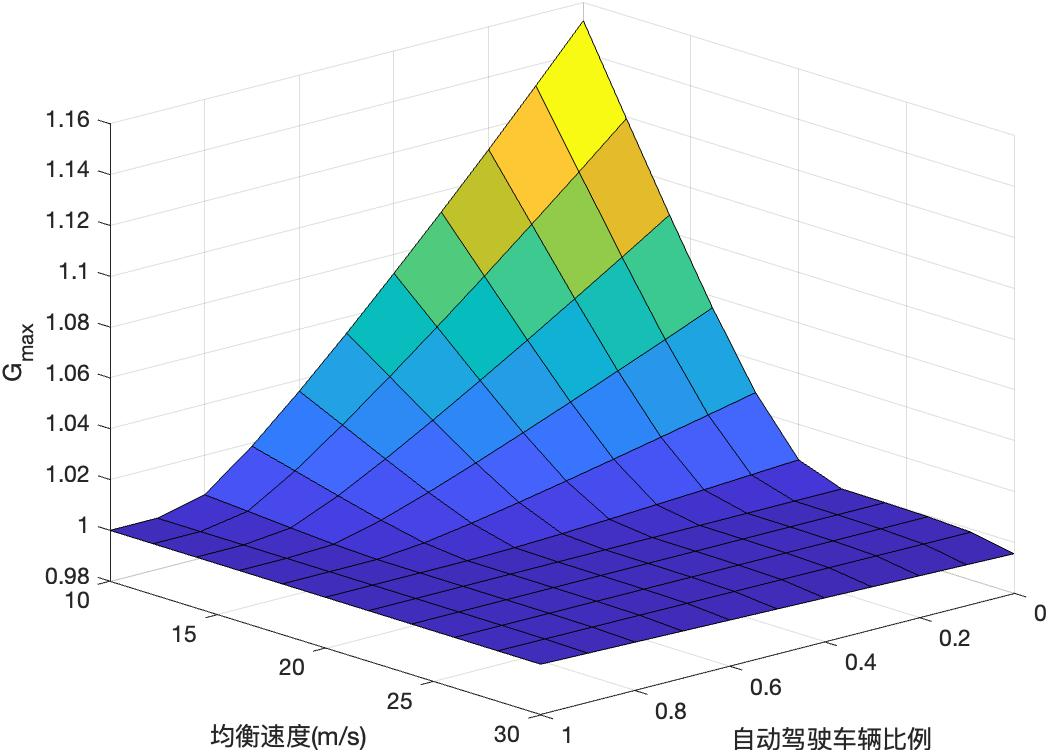
\includegraphics[width=0.9\linewidth]{chap04-Gmax.jpg}
    \caption{$G_{max}$函数图像}
    \label{fig:chap04-1}
\end{figure}

可以发现总体上,当固定自动驾驶车辆比例$p$,$G_{max}$随着初始均衡速度$v_e$的增大而减小;当固定初是均衡速度$v_e$,$G_{max}$随着自动驾驶车辆比例$p$的增大而减小。
因为$G_{max}$描述的是车队中车头受到的扰动到队尾的传递情况,所以可以认为$G_{max}$越大,车队的队列稳定性越差,反之,则相反。于是可以认为,对于一个混合车队,自动驾驶
车辆比例越大,初始的均衡速度越大,车队的队列稳定性越好。

另一方面,可以发现在选定的跟驰模型参数下,$G_{max}$的值多大于等于1,即对理论上不稳定的样本会有较好的描述,而由于稳定的样本的$G_{max}$取值集中在一个较小的区间,所以
在该指标下的区分度并不是很好。

下面通过仿真实验探究碰撞的发生与车队稳定性之间的关系。实验设计为:自动驾驶车辆比例$p$以0.1的步长遍历0到1,对于每一个$p$的取值,初始均衡速度以$2m/s$的步长遍历$10m/s$
到$30m/s$,对于每一组$(p, v_e)$取值,计算其$G_{max}$,并统计碰撞发生的频率。需要说明的是,即使确定了$p$和$v_e$的取值,车队仍有$\binom{10}{10\times p}$种排列,不同的排列
虽然$G_{max}$取值相同,但碰撞情况可能不同,这里的碰撞发生的频率就是指发生了碰撞的排列占所有排列的比例。

\begin{figure}
    \centering
    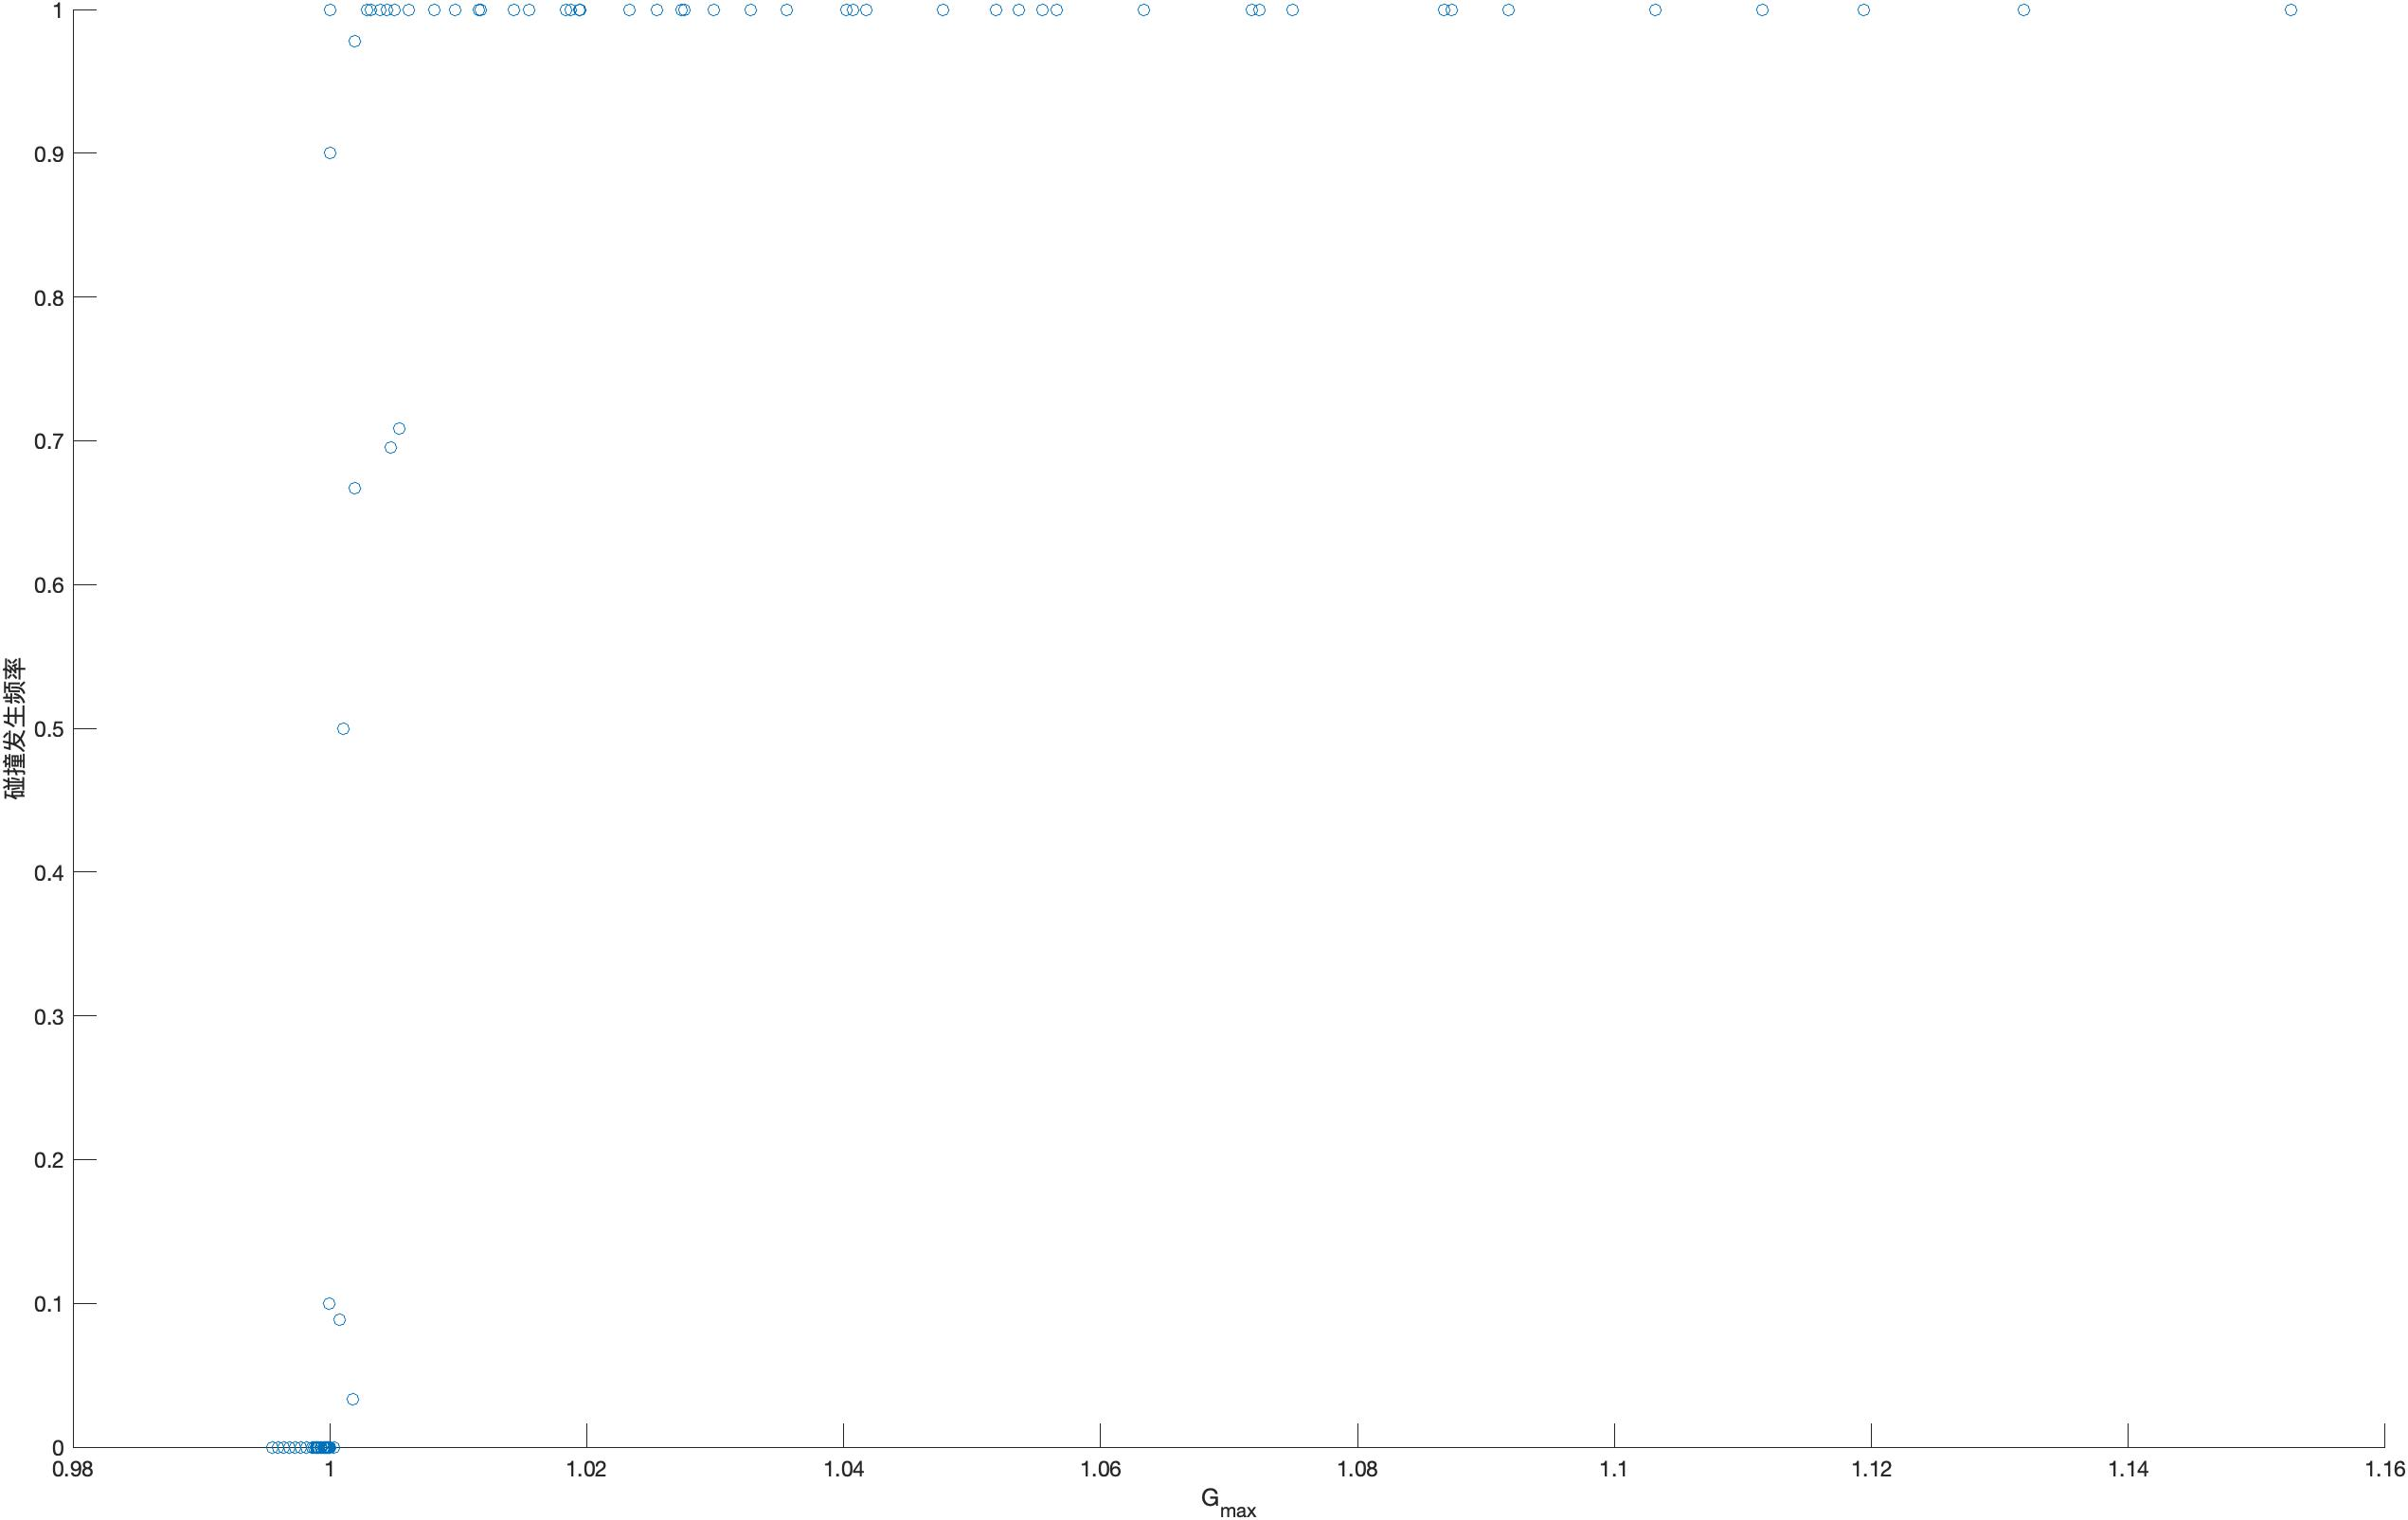
\includegraphics[width=1\linewidth]{chap04-crash-rate.jpg}
    \caption{碰撞频率与稳定性指标$G_{max}$的关系}
    \label{fig:chap04-2}
\end{figure}

实验得到结果如图\ref{fig:chap04-2}所示。可以发现总体上,$G_{max}$越大,碰撞发生的频率也越高,当$G_{max}$足够大时,几乎一定会发生碰撞,当$G_{max}$足够小时,几乎一定不会发生碰撞。
还有一个重要的结论是,理论上队列稳定($G_{max} < 1$)的车队也有可能发生碰撞,而理论上不稳定($G_{max} > 1$)的车队也并不是一定会发生碰撞,即发生碰撞与否并不取决于$G_{max}$的取值,
但与$G_{max}$有一定的关联。

通过图\ref{fig:chap04-2}还可以发现,发生碰撞并不是一个小概率事件,所以将发生碰撞的样本和不发生碰撞的样本分开讨论是有必要的。通过此图像也可以看出,
$G_{max} < 1$的样本多集中在一个较小的区间,而$G_{max} > 1$的样本则比较分散,这与对图\ref{fig:chap04-1}的分析是一致的。

\section{碰撞样本分析}

\subsection{稳定性指标选取}

对于发生了碰撞的样本,其对应的$G_{max}$多是大于1的,$G_{max} > 1$的样本则比较分散,所以用$G_{max}$作为碰撞样本的队列稳定性指标是比较合适的。

\subsection{碰撞风险指标选取}

在本课题中,有两个衡量车队碰撞风险(安全性)的指标。

一是追尾发生的时间$t_{crash}$,我们认为追尾事故发生得越早,车队整体越不安全。

二是发生追尾的车辆的下标$\mathrm{Index}_{crash}$,我们认为追尾事故发生得越靠近头车,车队整体越不安全。

\subsection{稳定性与碰撞风险关系探究}

首先探究追尾发生的时间$t_{crash}$与车队队列稳定性$G_{max}$之间的关系。与分析是否发生碰撞与车队的稳定性的关系时设计的实验一样,
对自动驾驶车辆比例$p$和初始均衡速度$v_e$进行遍历,挑选出发生了碰撞的样本,计算其对应的$G_{max}$,并统计追尾发生的时间。实验结果如图\ref{fig:chap04-3}所示。

\begin{figure}
    \centering
    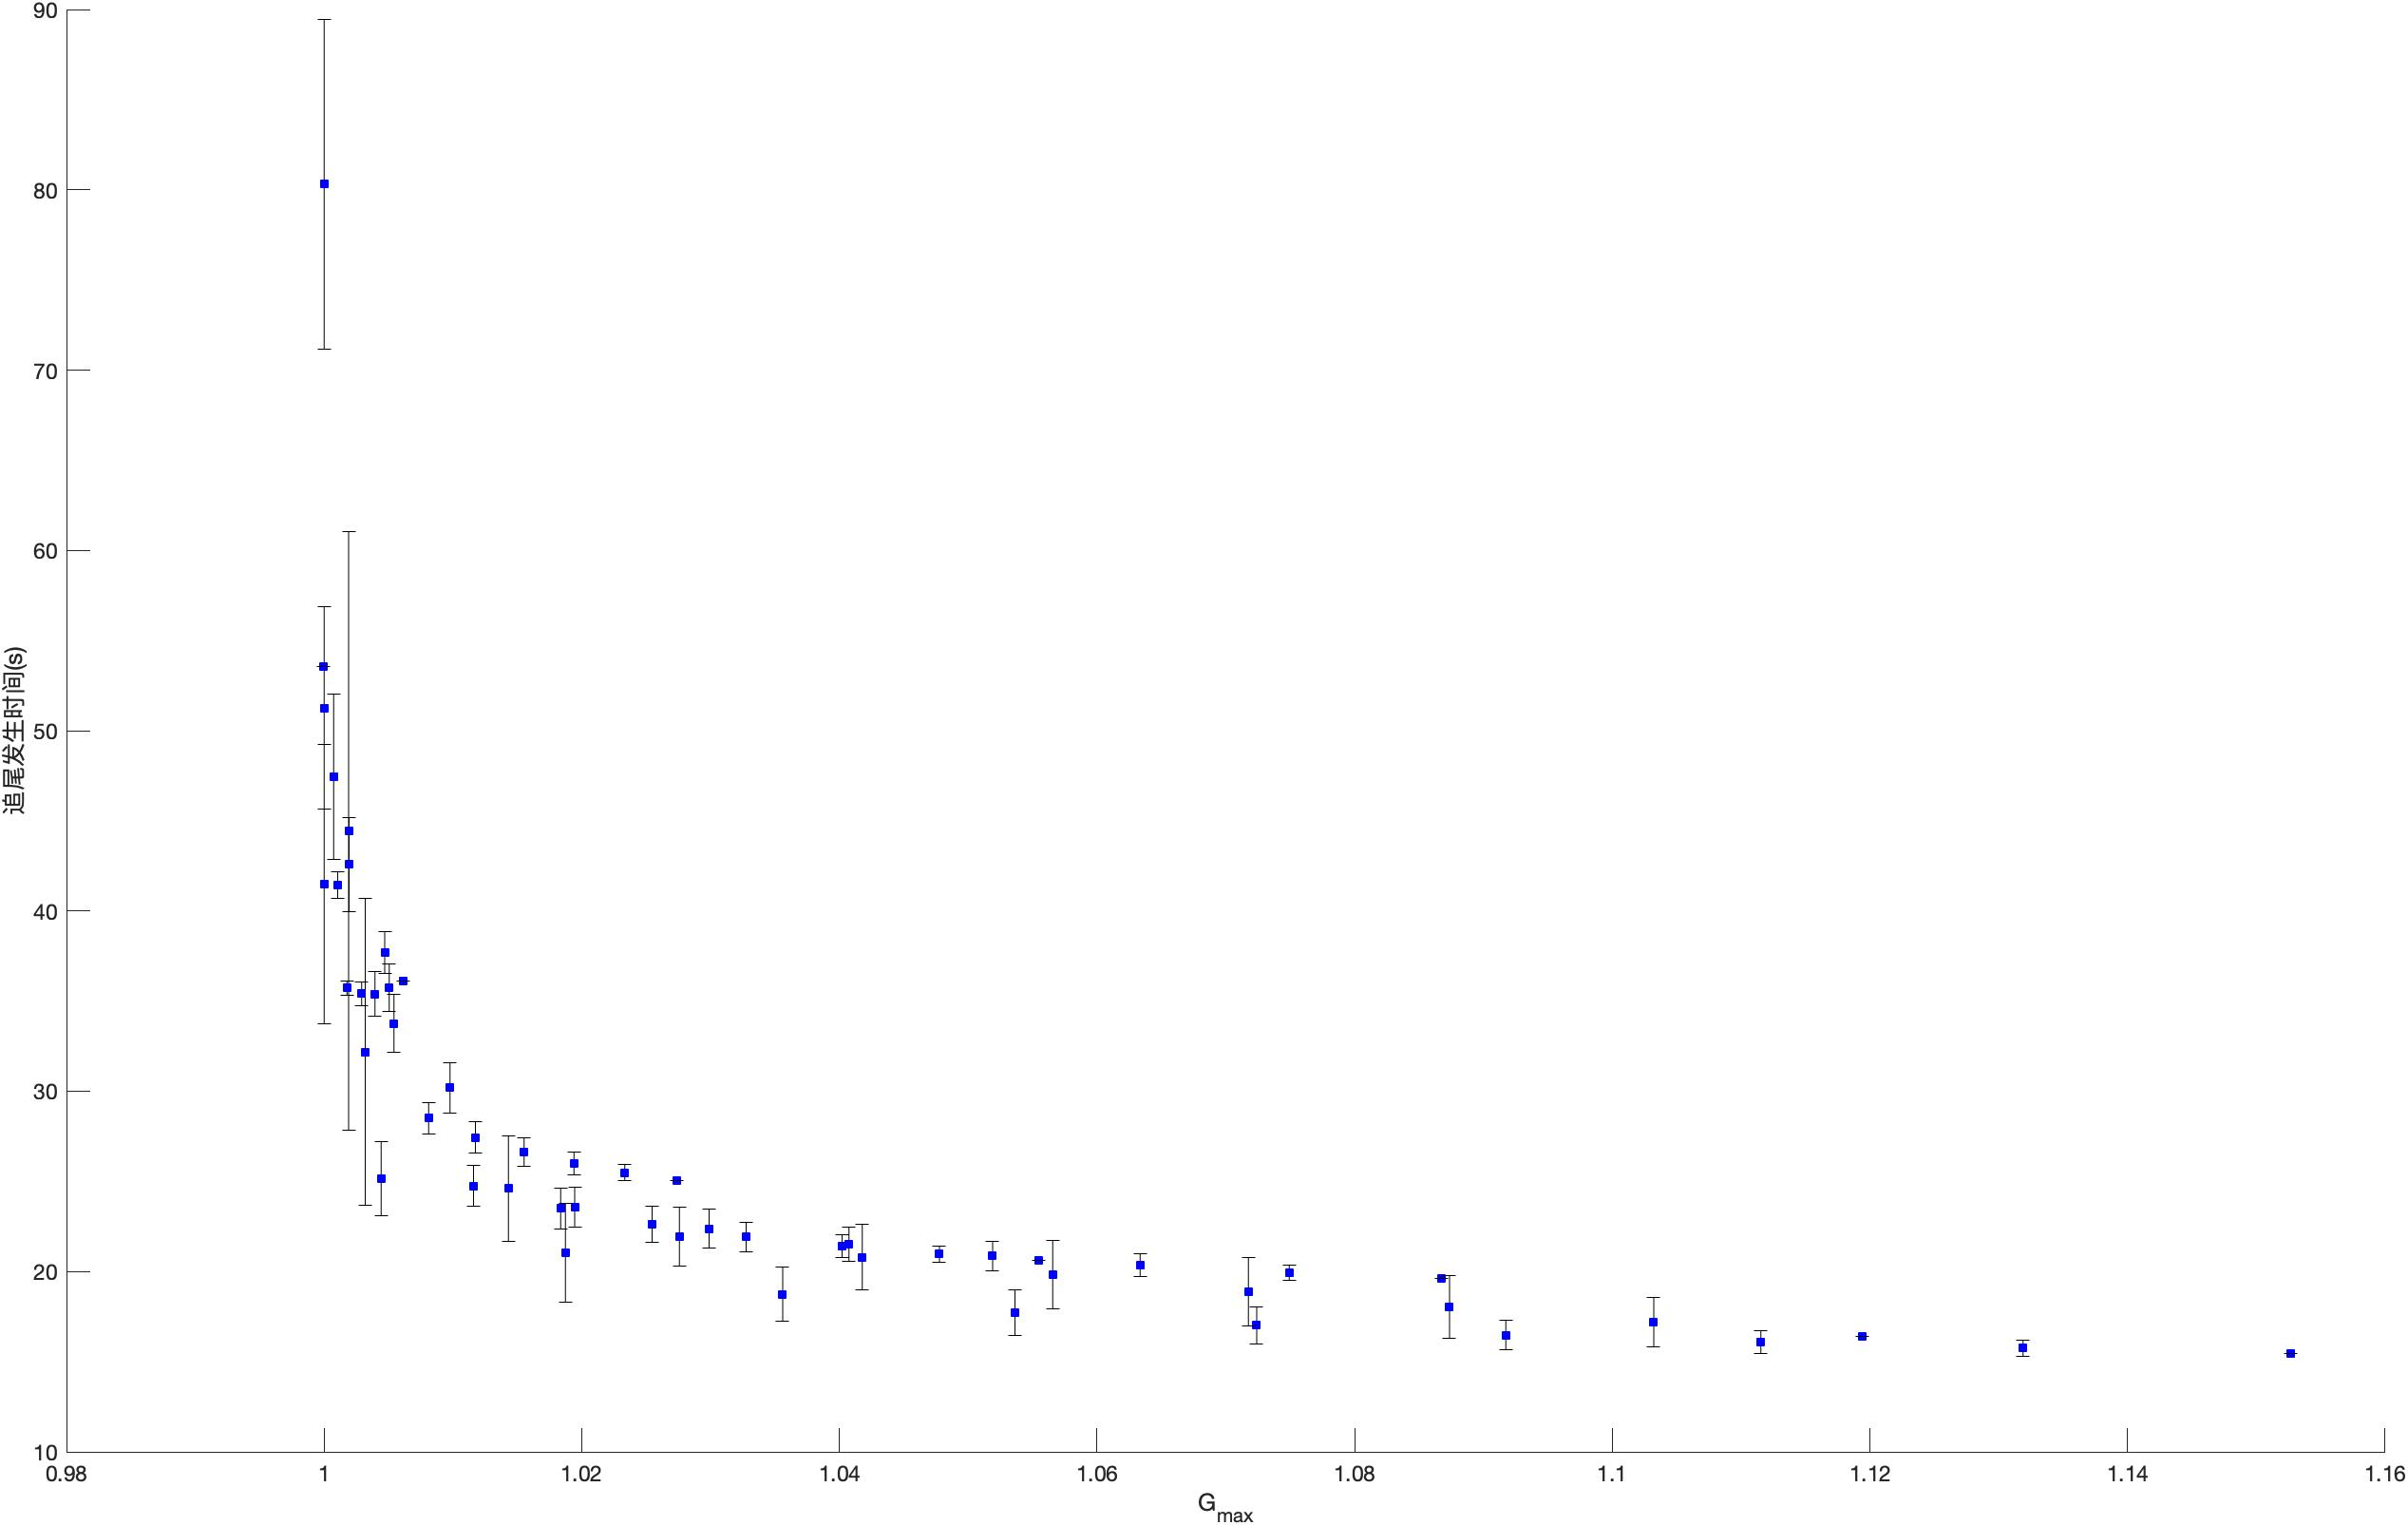
\includegraphics[width=1\linewidth]{chap04-t_crash.jpg}
    \caption*{Error bar代表标准差}
    \caption{追尾发生时间$t_{crash}$与稳定性指标$G_{max}$的关系}
    \label{fig:chap04-3}
\end{figure} 

可以观察到随着$G_{max}$的增大,碰撞发生的时间越小,即车队的队列稳定性越差,追尾发生的越快。其规律类似于反比例函数。此现象可以解释为:$G_{max}$越大,车队的队列稳定性越差,
扰动被放大的速度越快,碰撞就发生得越早。该关系是稳定性与碰撞风险在时间维度上的关系。

而通过发生追尾的车辆的下标$\mathrm{Index}_{crash}$则可以得到稳定性与碰撞风险在空间维度上的关系。如图\ref{fig:chap04-4}所示。

\begin{figure}
    \centering
    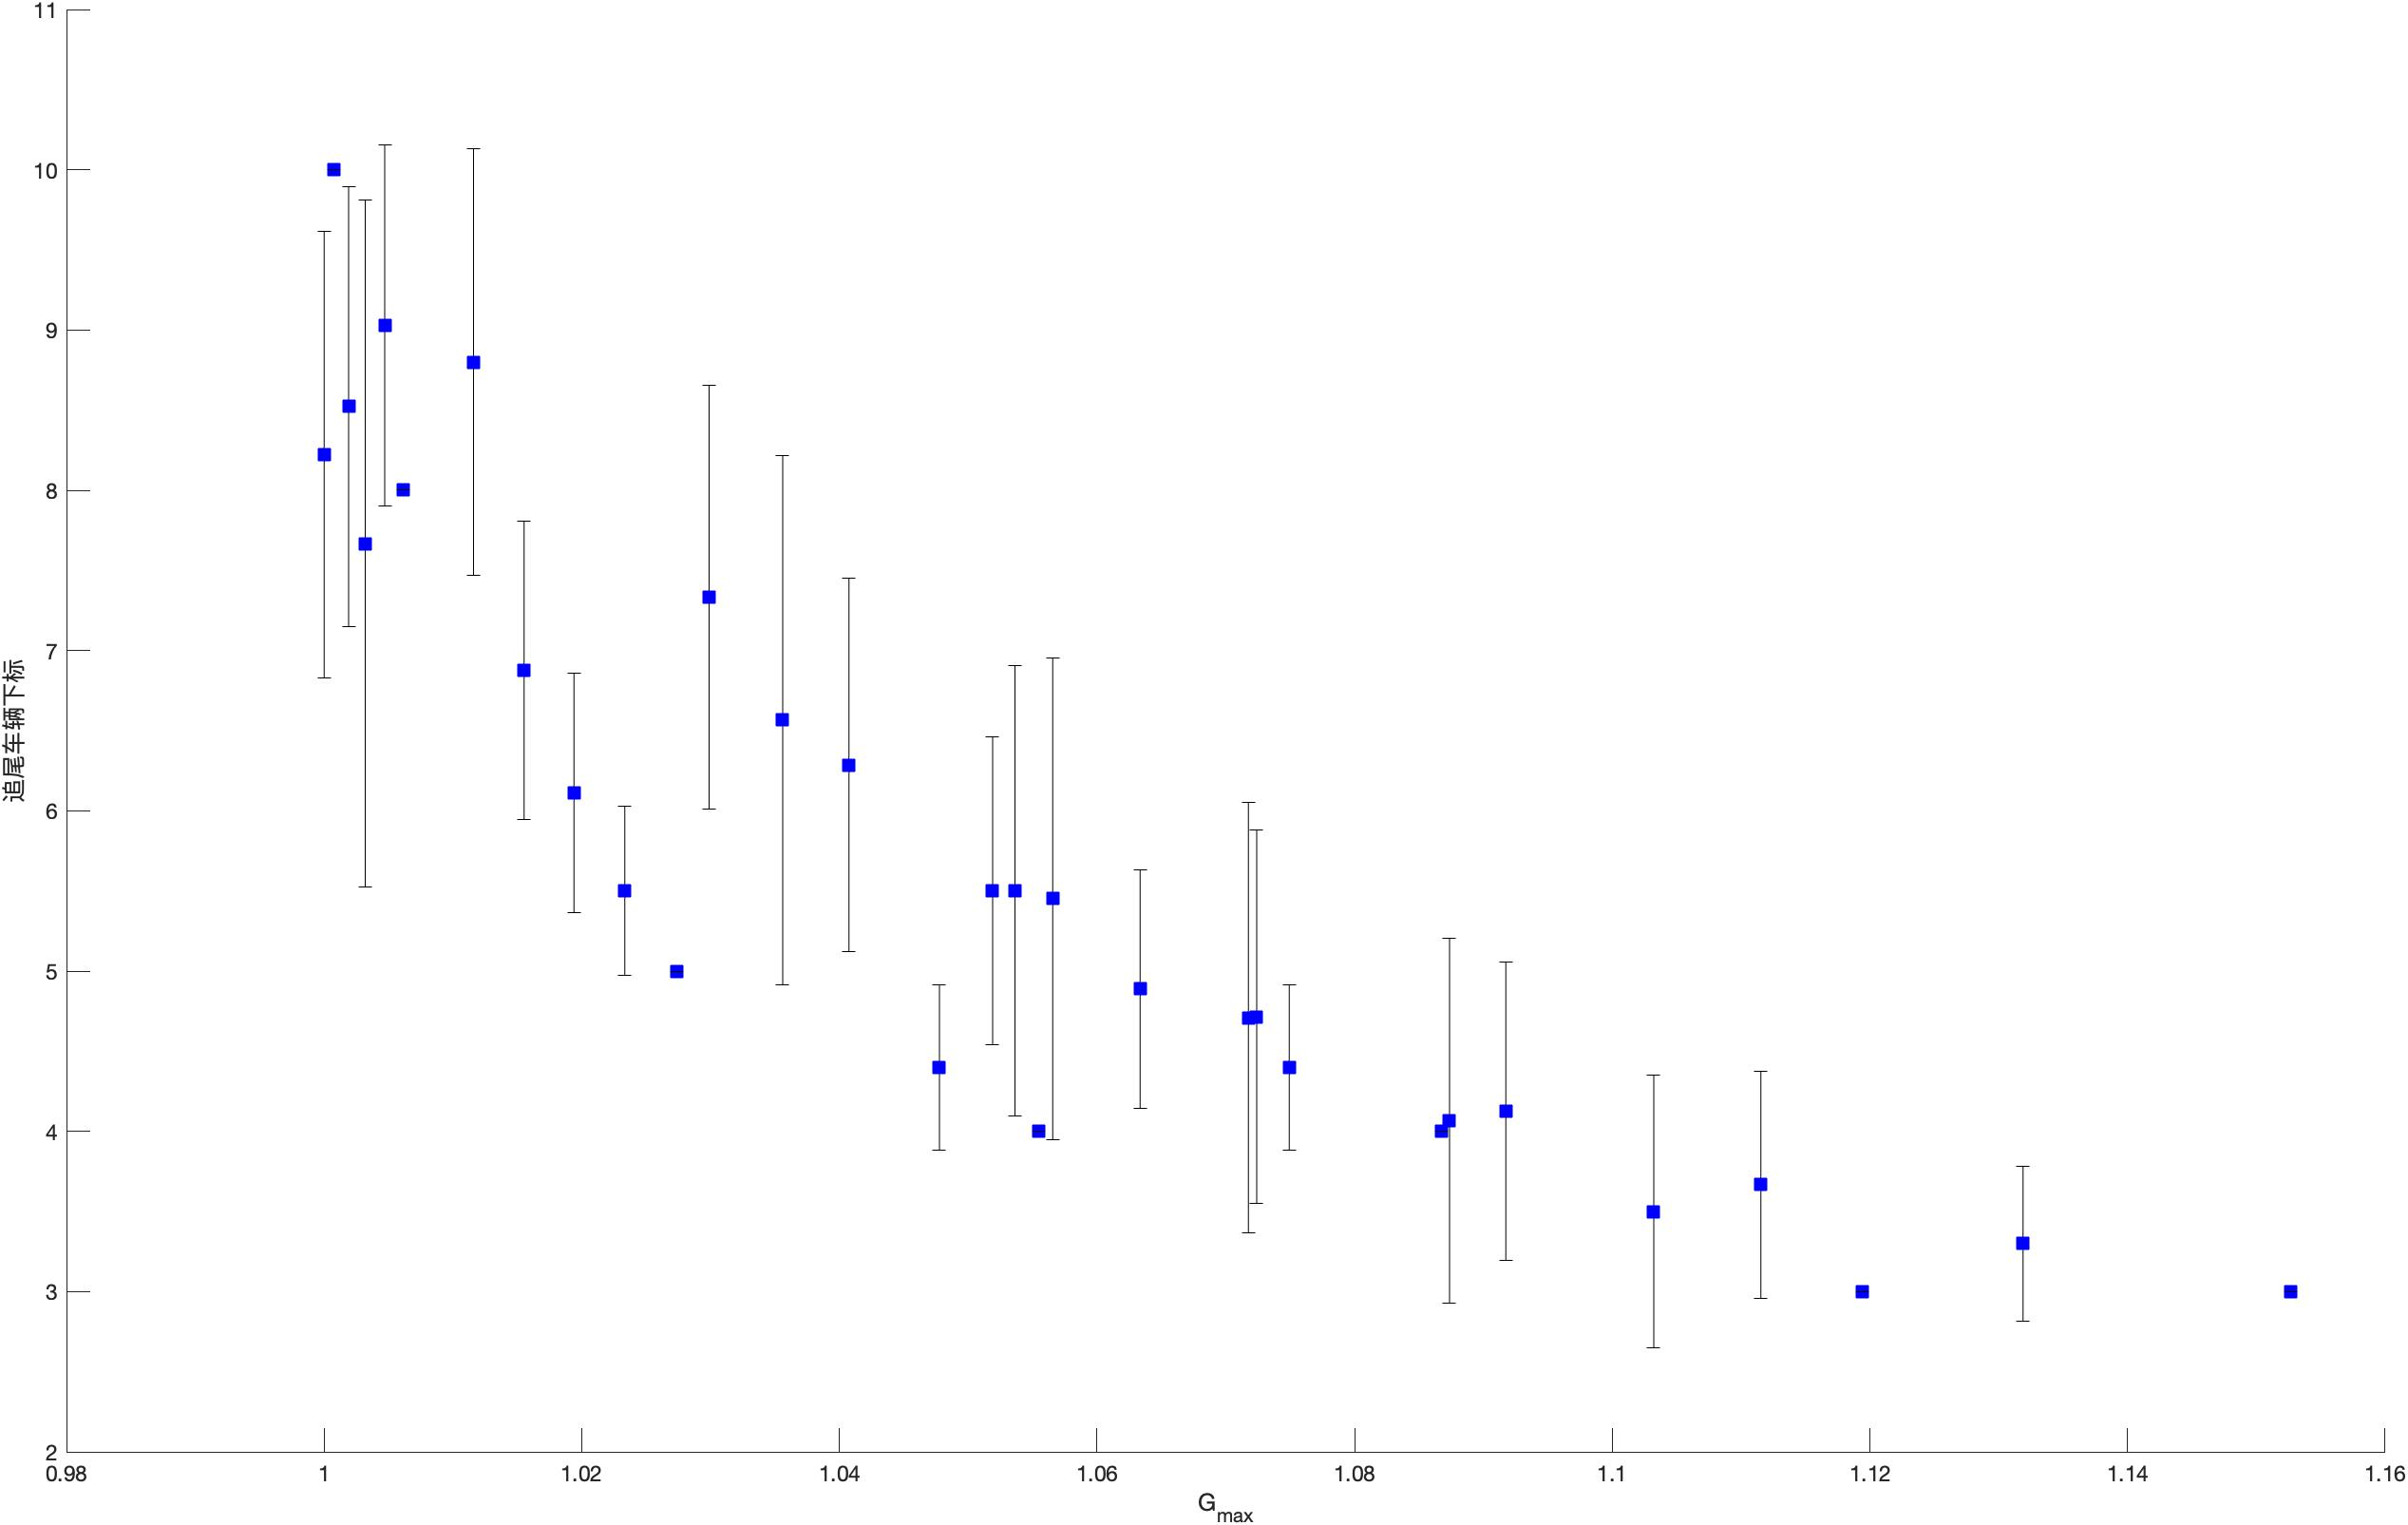
\includegraphics[width=1\linewidth]{chap04-crash_index.jpg}
    \caption*{Error bar代表标准差}
    \caption{追尾车辆下标$\mathrm{Index}_{crash}$与稳定性指标$G_{max}$的关系}
    \label{fig:chap04-4}
\end{figure} 

从图\ref{fig:chap04-4}中可能看出$\mathrm{Index}_{crash}$与$G_{max}$存在相关性。整体来看,$G_{max}$越大,$\mathrm{Index}_{crash}$越小,即车队队列稳定性越差,
碰撞发生得越靠前。这可以解释为:头车受到扰动后,扰动沿着车队传播,传递函数最大增益$G_{max}$越大,稳定性越差,扰动被放大的速度越快,碰撞发生得越靠前。

无论是从指标$t_{crash}$来看,还是从指标$\mathrm{Index}_{crash}$来看,都可以发现,车队的队列稳定性越差,车队的安全性越差。

在车队中,人工驾驶车辆和自动驾驶车辆对扰动的传递情况是不同的。通过\ref{sec:3.3}的仿真可以发现,在理想情况下,自动驾驶车辆会将前车的扰动略微放大,而扰动经过人工驾驶车辆则在不断
衰减;而对于模拟真实场景下的仿真,当给人类驾驶员引入$1.2s$的反应延迟后,似乎人工驾驶车辆也带来了不稳定的因素。下面就通过改变车队中车辆的排列,探究碰撞风险在车队中的演化机理。

\subsection{车队碰撞风险演化机理探究}
\label{sec:4.2.4}

\subsubsection{空间分布指标选取}
\label{sec:4.2.4.1}

参考王大均在空间分布指标选取方面的工作\cite{wang2021auto},在对自动驾驶车辆在车队中的空间分布研究时,主要关注两个指标。

一是自动驾驶车辆整体靠近头车的程度。该指标的意义在于,如果自动驾驶车辆整体越靠前,那么扰动最先由自动驾驶车辆传递,通过对追尾车辆下标的分析,可以分析发生碰撞的下标与自动驾驶整体分布的下标之间的关系。

二是自动驾驶车辆的分散程度。在指标的意义在于,如果自动驾驶车辆会放大扰动,人工驾驶车辆可以衰减扰动,那么将自动驾驶车辆分散排布在车队中可能会比将自动驾驶车辆集中在一起更加安全。

通过对同一稳定性的不同车辆排列进行仿真实验,可以探究,下面对两个指标的计算方式进行介绍。 \\

\noindent \textbf{(1)队首聚集度}

队首聚集度($\mathrm{Index}_{front}$)衡量了车队中自动驾驶车辆整体靠近头车的程度。记车队中共有$n$辆跟随车辆,其中有$m$辆是自动驾驶车辆,每一辆自动驾驶车辆在车队中的下标为$C = (c_1, c_2, \cdots, c_m)$,同时记$C(i) = c_i$,
那么队首聚集度的计算公式为

\begin{equation}
    \begin{cases}
      temp = \frac{\sum_{i=1}^{m}[C(i) - 1 ]}{nm - \sum_{i=1}^{m}i} \\
      \mathrm{Index}_{front} = \frac{temp - \min(temp)}{\max(temp) - \min(temp)}
    \end{cases}
    \label{eq:chap04-2}
\end{equation}

在式(\ref{eq:chap04-2})中进行了归一化,指标值域为$[0,1]$,且指标取值越小说明说明自动驾驶车辆总体分布越靠近头车。在使用该指标时,需要车队中至少有1辆自动驾驶车辆。 \\

\noindent \textbf{(2)分散均匀度}

分散均匀度($\mathrm{Index}_{disp}$)衡量了车队中自动驾驶车队整体的分散程度。关于车队的描述与队中聚集度相同,分散均匀度的计算方式为

\begin{equation}
    \begin{cases}
      temp = \frac{\sum_{i=1}^m [C(i)-C(i-1)]^{-1}}{m-1} \\
      \mathrm{Index}_{disp} = \frac{temp - \min(temp)}{\max(temp) - \min(temp)}
    \end{cases}
    \label{eq:chap04-3}
\end{equation}

同样,在式(\ref{eq:chap04-3})中也进行了归一化,指标值域为$[0,1]$,且指标取值越小说明说明自动驾驶车辆总体分布越分散、越均匀。在使用该指标时,需要车队中至少有2辆跟驰车辆。

\subsubsection{仿真实验结果分析}

实验设计如下:固定自动驾驶车辆比例$p=0.5$,初始均衡速度$v_e = 15m/s$。通过计算可以发现该取值下车队理论上是队列不稳定的,通过图\ref{fig:chap04-2}可以看出在该稳定性下车队非常容易发生碰撞。
实验的其他设置与前文中的实验保持一致。

实验结果如图\ref{fig:chap04-5}所示。

\begin{figure}
    \centering
    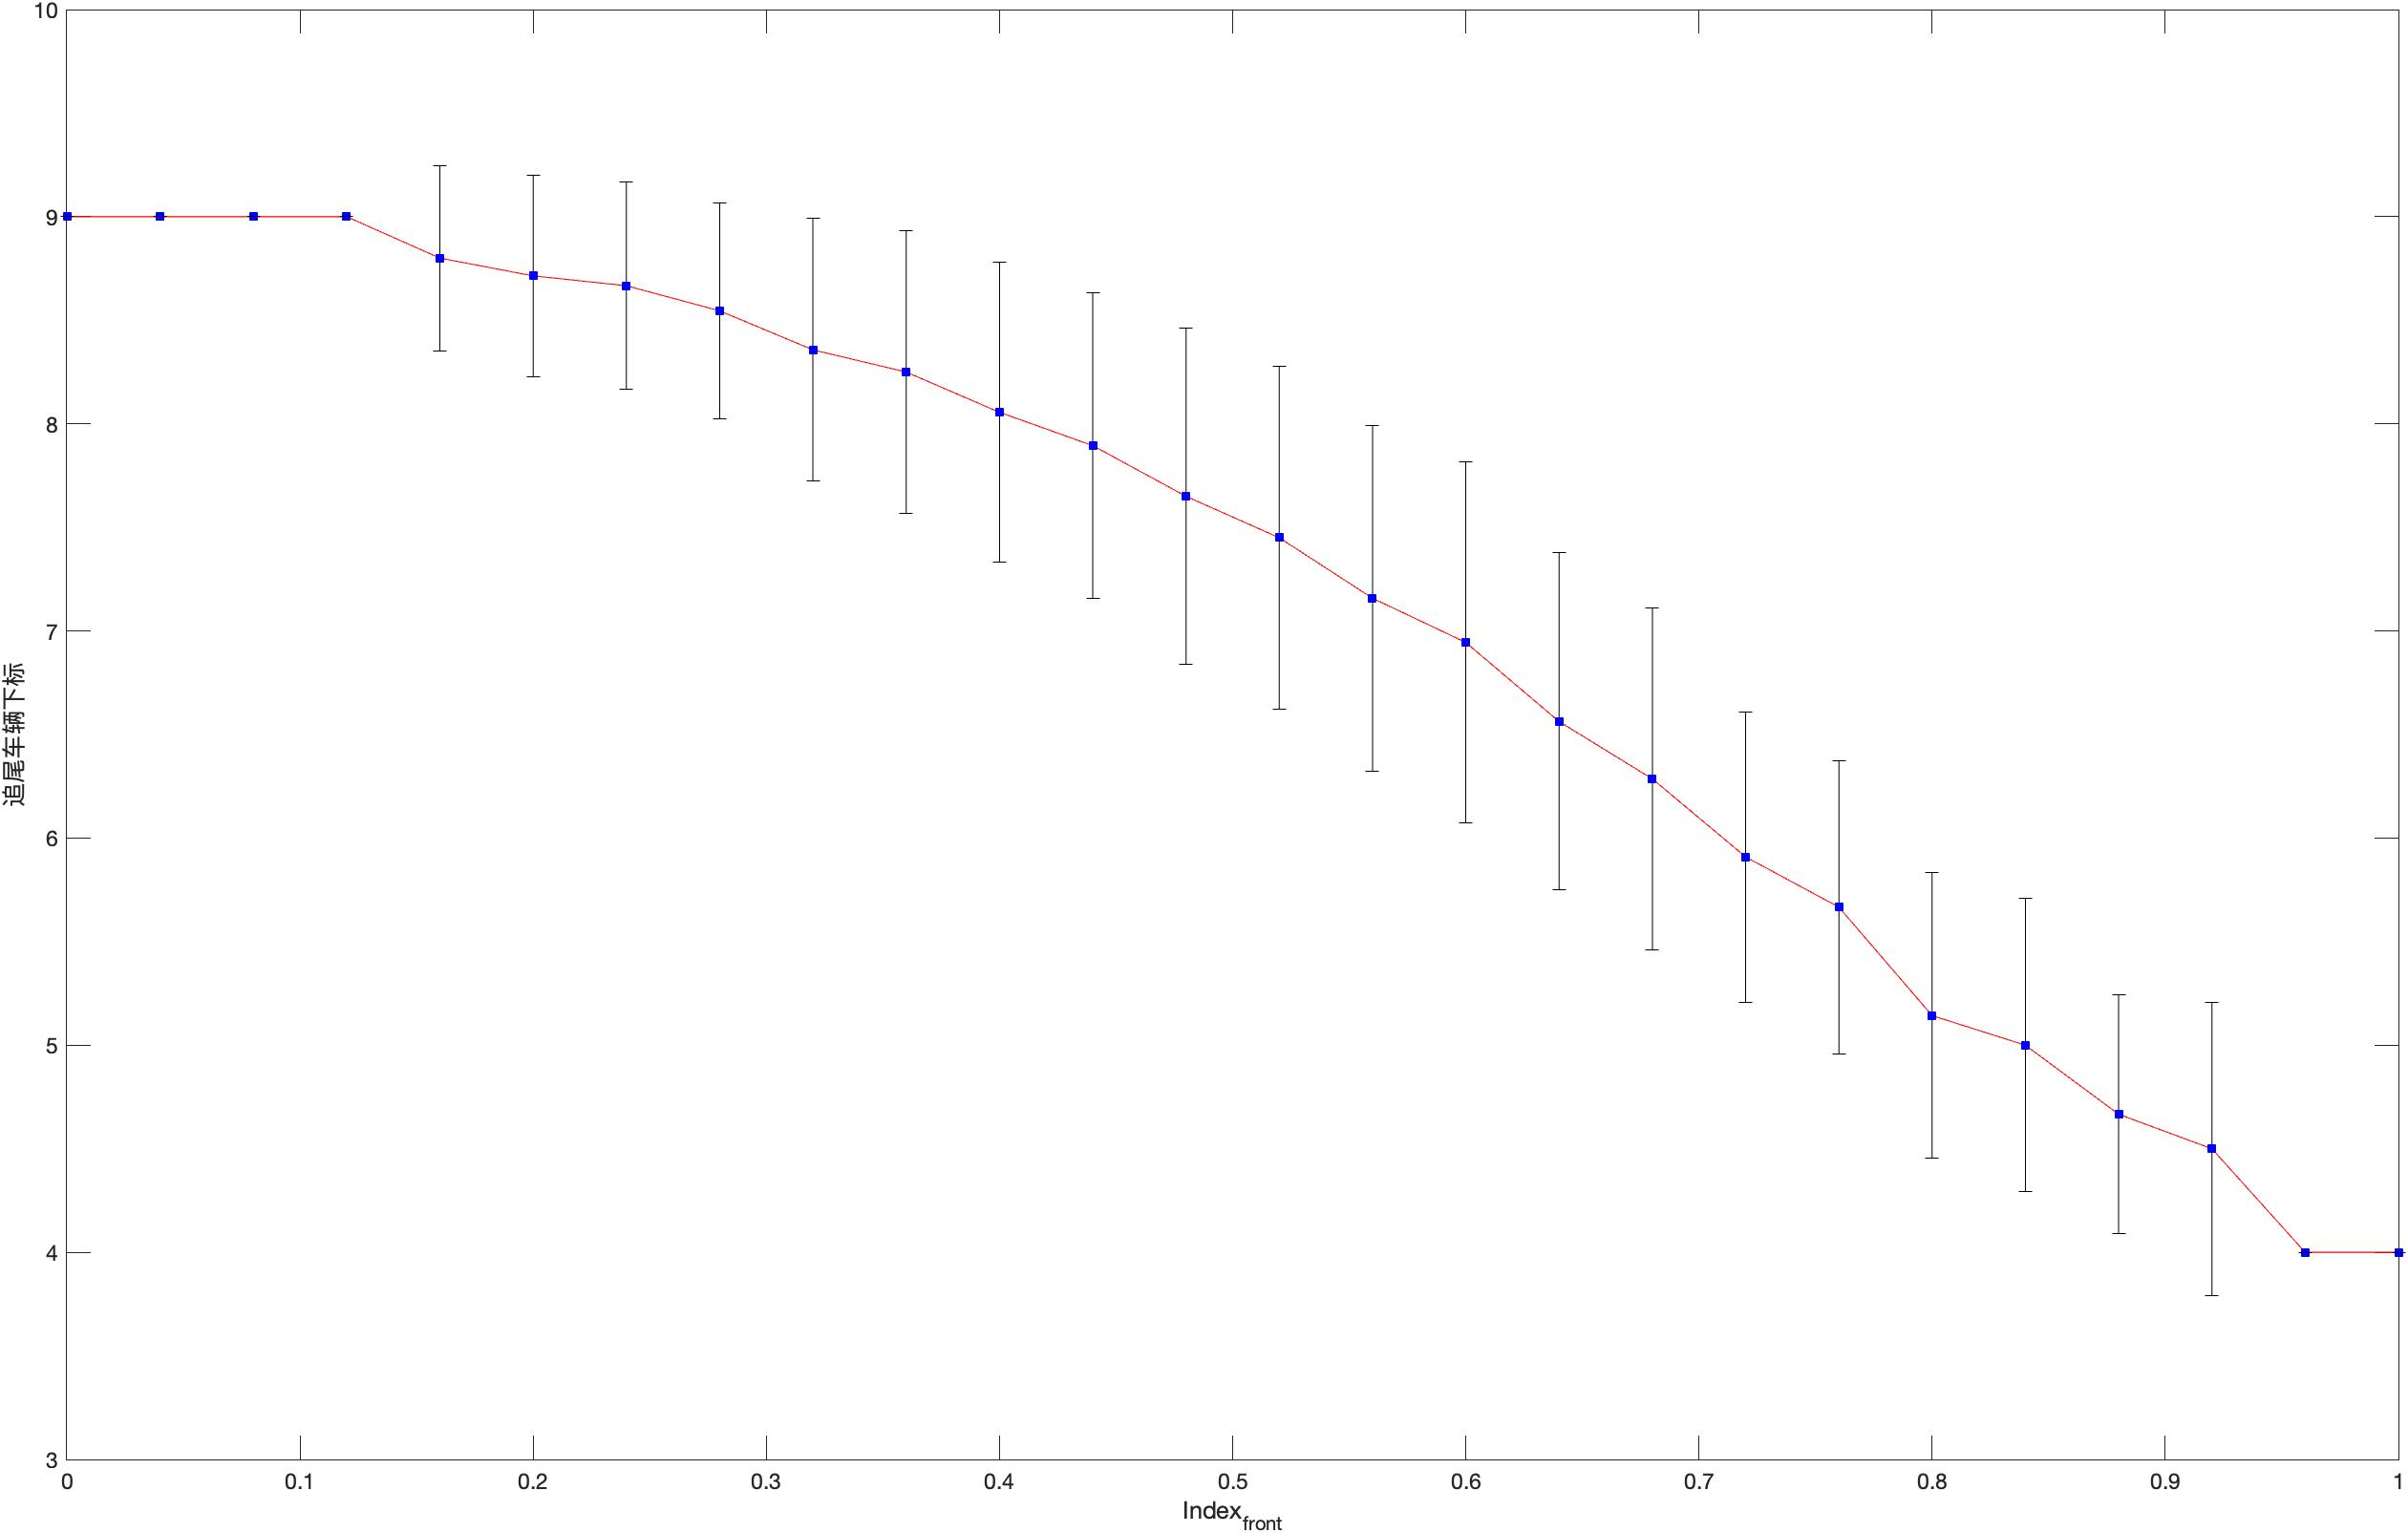
\includegraphics[width=1\linewidth]{chap04-front-crash.jpg}
    \caption*{Error bar代表标准差}
    \caption{队首聚集度与追尾车辆下标的关系}
    \label{fig:chap04-5}
\end{figure} 

可以看出队首聚集度与追尾车辆的下标是负相关的,且存在一定的线性关系。计算二者的Pearson相关系数为$-0.8281$,对于向量$\mathrm{X}$和向量$\mathrm{Y}$,其Pearson相关系数的计算公式如式(\ref{eq:chap04-4})。

\begin{equation}
    r = \frac{\mathbb{E}\mathrm{XY}-\mathbb{E}\mathrm{X}\mathbb{E}\mathrm{Y}}{\sqrt{\mathbb{E}\mathrm{X^2}-(\mathbb{E}\mathrm{X})^2}\sqrt{\mathbb{E}\mathrm{Y^2}-(\mathbb{E}\mathrm{Y})^2}}
    \label{eq:chap04-4}
\end{equation}

从图\ref{fig:chap04-5}可以看出,当队首聚集度指标$\mathrm{Index}_{front}$越大,追尾车辆下标越小,即自动驾驶车辆整体越远离头车,追尾发生在越靠近头车的地方,即追尾总是倾向于发生在人工驾驶车辆处。这也可以说明人工驾驶车辆会给车队带来更大的碰撞风险。

为了获得更加清晰的碰撞风险演化机理,将自动驾驶车辆比例$p$以0.1的步长遍历0到1,对于每一个$p$的取值,初始均衡速度以$2m/s$的步长遍历$10m/s$
到$30m/s$,对实验中追尾车辆及其前后车的车辆种类进行了统计,结果如表\ref{tab:chap04-2}所示。

\begin{table}
    \centering
    \caption{追尾车辆及其前后车车辆种类统计}
    \begin{tabular}{ccl}
      \toprule
      追尾车辆类型                 &                                &  数量及比例  \\
      \midrule
      \multirow{4}{*}{AV : 999 (19.09\%)}         &    \multirow{2}{*}{前车类型}    &   AV : 47 (4.70 \%)    \\
                                 &                                       &   HV : 952 (95.30 \%)   \\
      \cline{2-3}
                                 &    \multirow{2}{*}{后车类型$^*$}    &   AV : 508 (50.58 \%)    \\
                                 &                                &   HV : 247 (24.72 \%)   \\       
      \hline
      \multirow{4}{*}{HV : 4235 (80.91\%)}        &    \multirow{2}{*}{前车类型}    &   AV : 1753 (41.39 \%)    \\
                                 &                                &   HV : 2482 (58.61 \%)  \\      
      \cline{2-3}
                                 &    \multirow{2}{*}{后车类型$^*$}    &   AV :1948 (46.00 \%)  \\
                                 &                                &   HV : 2245 (53.01 \%)  \\     
      \bottomrule
    \end{tabular}
    \caption*{*由于有部分追尾车辆已是尾车,所以后车类型会出现比例和小于1的情况}
    \label{tab:chap04-2}
  \end{table}

可以发现追尾车辆大多是人工驾驶车辆造成的,占到了$80.91\%$,这与图\ref{fig:chap04-5}呈现的追尾总是倾向于发生在人工驾驶车辆处的规律是吻合的。通过观看可视化的仿真过程,发现人工驾驶的追尾多是由于人工驾驶车辆减速不及时造成的,造成这一现象的一个原因可能是在仿真时给人工驾驶员设置了$1.2s$的反应延迟,另一个可能原因是扰动在人工驾驶车辆传递过程中衰减的速度较慢,即相比自动驾驶车辆,人工驾驶车辆很有效地抵抗扰动,造成了较大的碰撞风险。

对被追尾车辆(即表中的前车)的类型进行分析,无论是人工驾驶车辆,还是自动驾驶车辆,其追尾的多是人工驾驶车辆,这一现象对于自动驾驶车辆更为明显,人工驾驶车辆占到自动驾驶车辆追尾车辆的$95.30\%$,这更能说明人工驾驶车辆对扰动的抵抗能力不是很强,当自动驾驶车辆跟驰自动驾驶车辆时,碰撞风险会变得更大,也很容易发生追尾事故。同时表中也列出了追尾车辆后车的类型,但由于无论是人工驾驶车辆,还是自动驾驶车辆,其跟驰模型都没有考虑后车,所以此处就不分析后车类型的分布情况了。

同时,也统计了队首聚集度与追尾发生时间之间的关系,如图\ref{fig:chap04-6}所示。可以发现二者也有很好的线性关系,其Pearson相关系数为$-0.7950$。队首聚集度越大,自动驾驶车辆整体越远离头车,扰动首先由人工驾驶车辆传递,由于人工驾驶车辆会引入更大的碰撞风险,所以碰撞也会更早地发生。

\begin{figure}
    \centering
    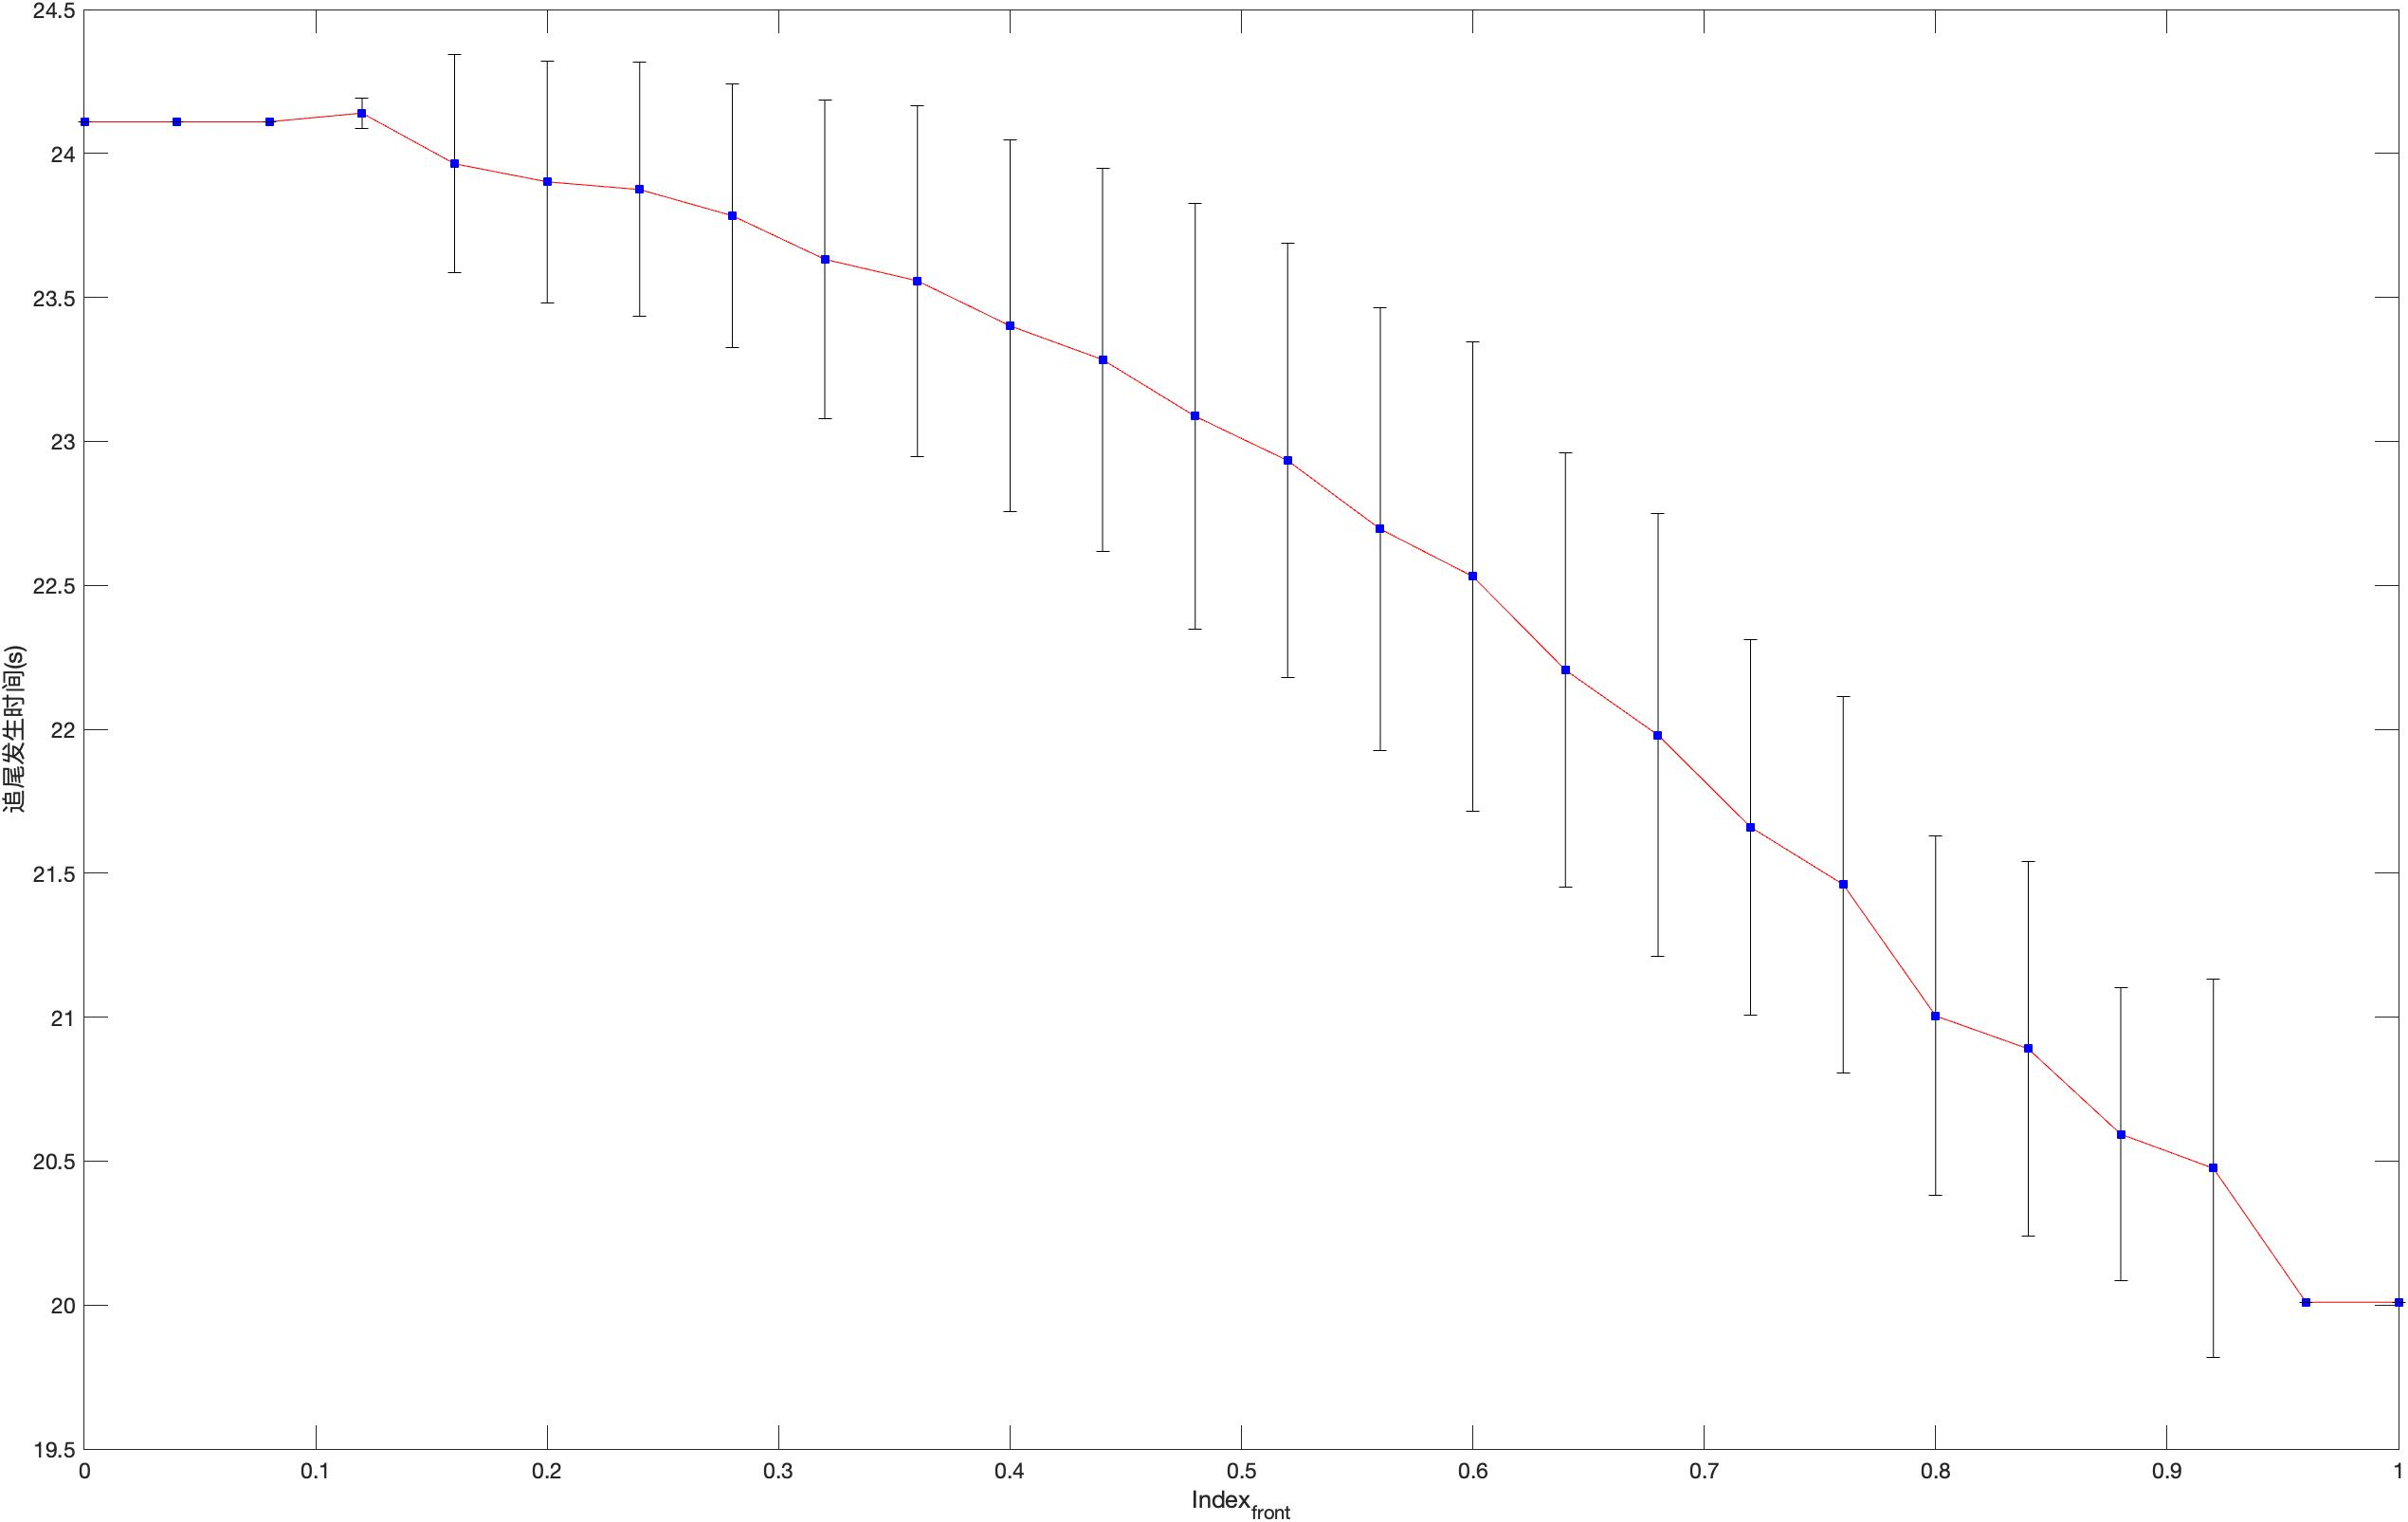
\includegraphics[width=1\linewidth]{chap04-front-time.jpg}
    \caption*{Error bar代表标准差}
    \caption{队首聚集度与追尾发生时间的关系}
    \label{fig:chap04-6}
\end{figure} 

另一个空间分布指标是分散均匀度,与分析队首聚集度时设计的实验相同,这里也固定人工驾驶车辆比例为$0.5$,初始均衡速度为$15m/s$,统计实验过程中追尾的下标与发生的时间,结果如图\ref{fig:chap04-7}所示。

\begin{figure}
    \centering
    \subcaptionbox{分散均匀度与追尾发生时间的关系 \label{fig:chap04-7-1}}
      {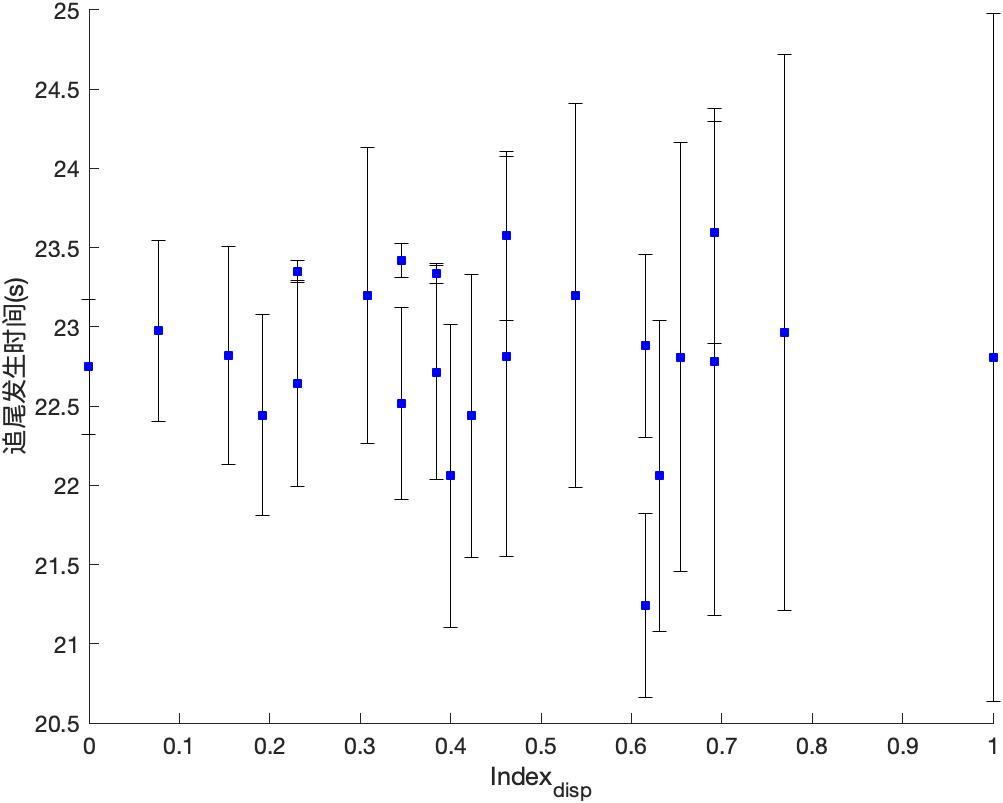
\includegraphics[width=0.49\linewidth]{chap04-disp-time.jpg}}
    \subcaptionbox{分散均匀度与追尾车辆下标的关系 \label{fig:chap04-7-2}}
      {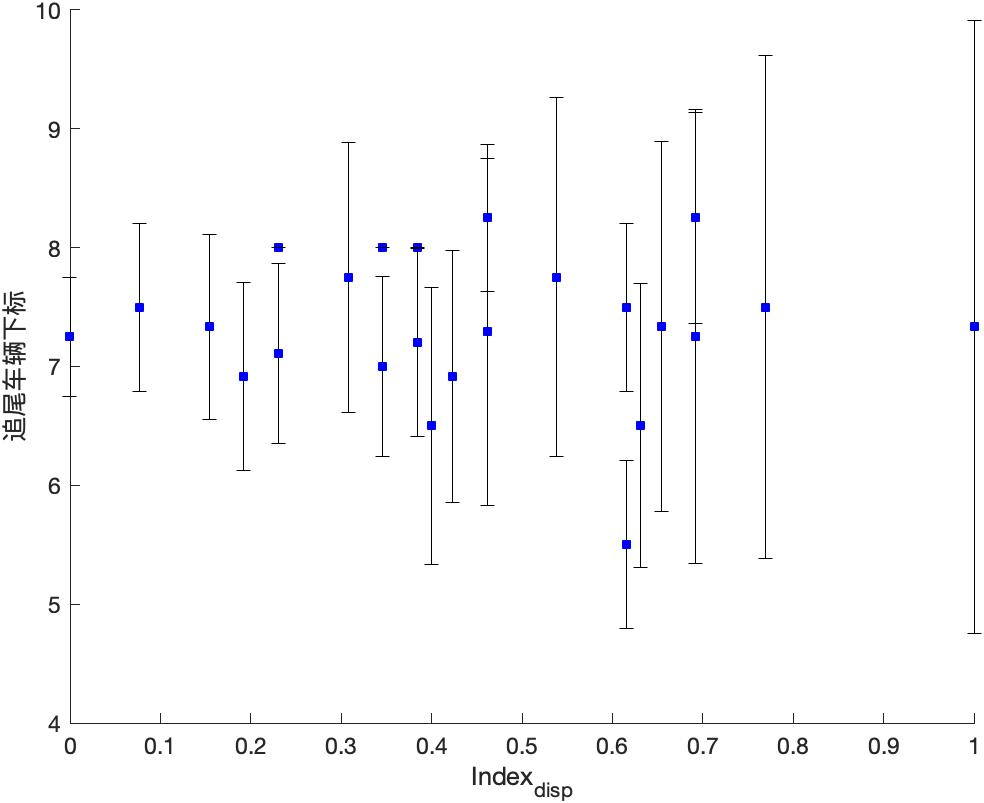
\includegraphics[width=0.49\linewidth]{chap04-disp-index.jpg}}
      \caption{分散均匀度与碰撞风险关系分析}
    \label{fig:chap04-7}
  \end{figure}

可以发现分散均匀度与追尾车辆下标以及追尾发生时间均没有明显关系,这说明自动驾驶车辆在车队中的分散程度并不会影响车队的碰撞风险大小。

\section{非碰撞样本分析}

\subsection{稳定性指标选取}

 与碰撞的样本不同,非碰撞的样本大多是理论上队列稳定的样本。由之前的分析得到,稳定样本的车队传递函数无穷范数$G_{max}$集中在一个很小的区间内,区分度不大,所以不适合用$G_{max}$作为非碰撞样本的队列稳定性指标。

 一个衡量一个系统稳定程度常用的指标是该系统受到扰动后,恢复到稳态所需要的时间,我们可以将该概念运用到对非碰撞样本队列稳定性的描述上。我们将从车队受到扰动开始,到车队中每一辆车都恢复到初始均衡速度的$\pm 5\%$范围内为止(并且从此之后各车的速度都保持在均衡速度的$\pm 5\%$以内)的时间称为车队的恢复时间,记作$t_{stable}$。$t_{stable}$越大,车队就越不稳定;反之,车队越稳定。

 值得说明的是,对于虽然没有发生碰撞,但在仿真的$500s$时间内没有达到稳定的样本,用$t_{stable}$这一指标并没有意义,通过统计发现这样的样本是极少数,所以在这一小节中,主要对没有发生碰撞,且在仿真的$500s$恢复的稳态的样本进行分析。

\subsection{碰撞风险指标选取}

由于研究的对象是没有发生碰撞的样本,所以用潜在危险时间(Potential Dangerous Time, PDT)比例来描述车队的碰撞风险。是否存在潜在危险的判断依据如式(\ref{eq:chap04-5})所示。

\begin{equation}
    \increment{x_n} \geqslant A + B - (C - l_{n-1})
    \label{eq:chap04-5}
\end{equation}
其中各变量参数如表\ref{tab:chap01-9}所示。

在仿真的$500s$中,存在潜在危险的时间占总时间的比例称为潜在危险时间比例。

\subsection{稳定性与碰撞风险关系探究}

仿真实验设计如下:以$0.1$的步长对自动驾驶车辆比例$p$进行遍历,对于每一个自动驾驶车辆比例,再以$2m/s$的步长对初始均衡速度进行遍历,将每一次仿真时间的结果进行统计。

图\ref{fig:chap04-8}所示是队列稳定性指标$t_{stable}$与潜在危险时间比例之间的关系。

\begin{figure}
    \centering
    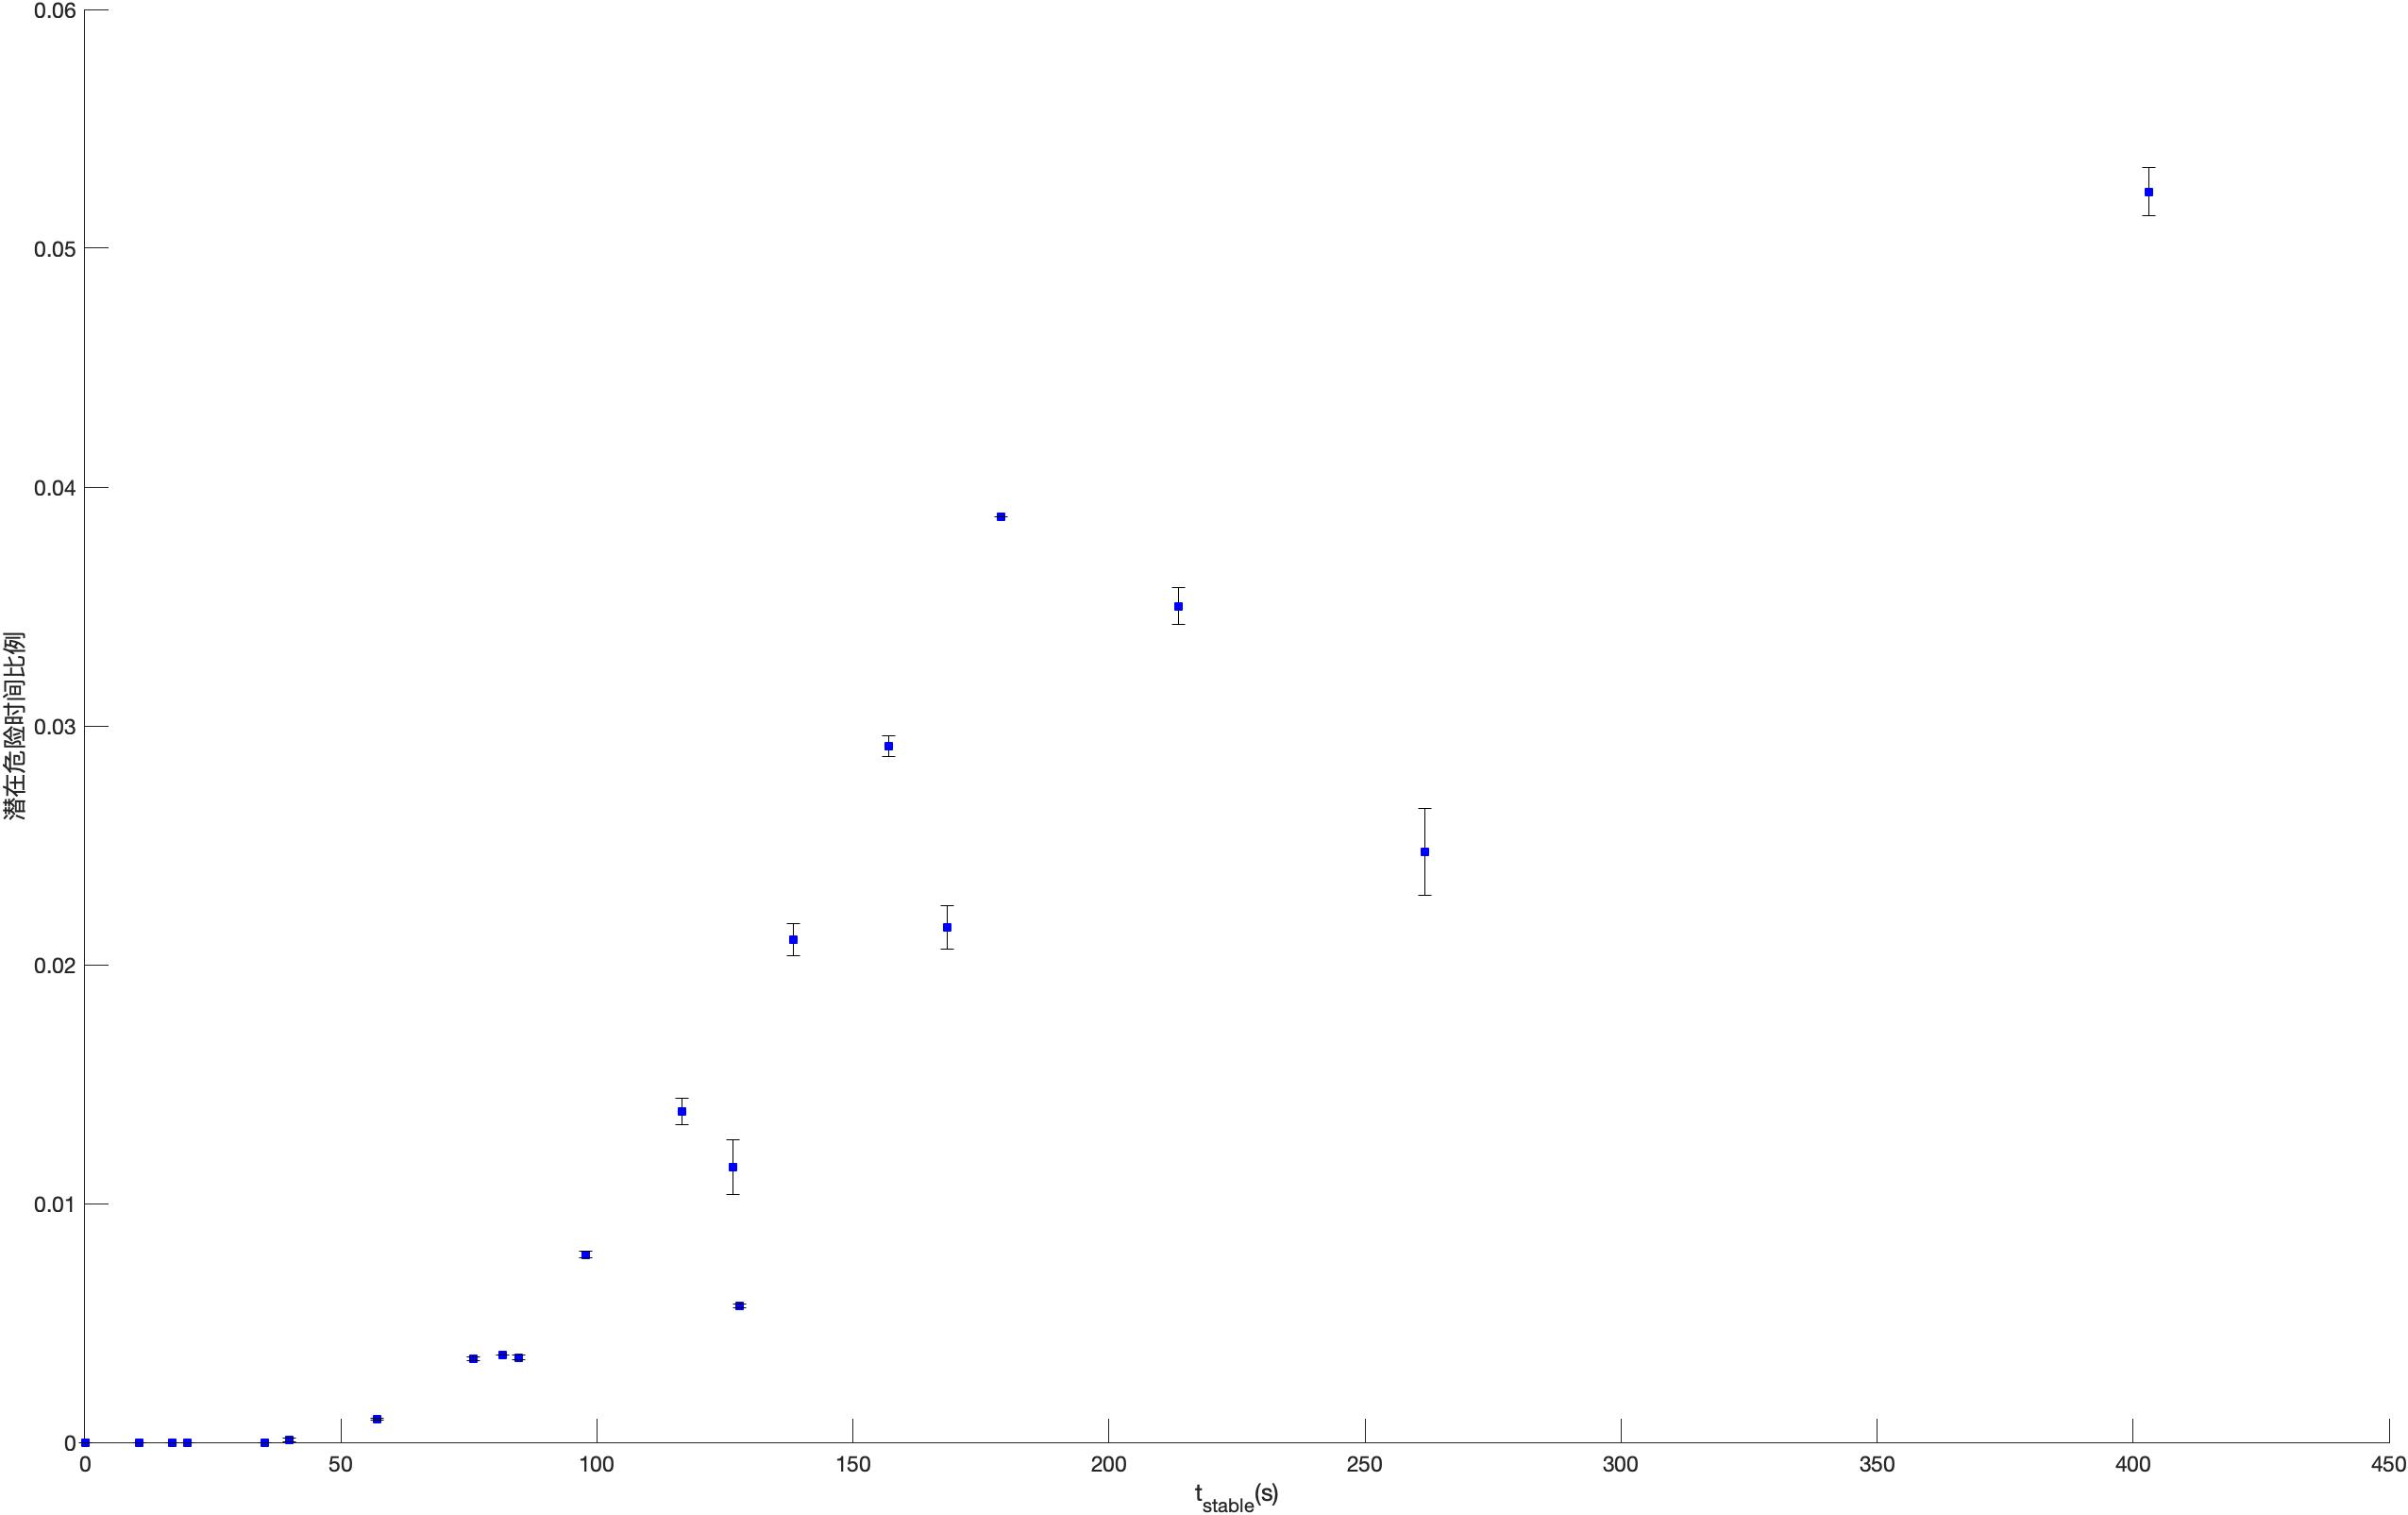
\includegraphics[width=1\linewidth]{chap04-PDT-tstable.jpg}
    \caption*{Error bar代表标准差}
    \caption{潜在危险时间比例与稳定时间的关系曲线}
    \label{fig:chap04-8}
\end{figure} 

可以发现潜在危险时间比例与稳定时间存在明显的相关性,稳定时间$t_{stable}$越小,车队的队列稳定性越好,车队中存在的潜在危险也越少。

在$t_{stable}$较小时(比如小于$50s$),车队能够迅速恢复稳定,此时车队中几乎不存在潜在危险,扰动给车队带来的影响较小;当$t_{stable}$较大时(比如大于$50s$),随着$t_{stable}$的增大,潜在危险时间比例也会增大,二者的Pearson相关系数达到了0.9476,说明二者有很强的相关性,并且可以观察到标准差比较小。

\subsection{车队碰撞风险演化机理研究}

在\ref{sec:4.2.4}中,探究了车队中发生了碰撞的情况下,车队中碰撞风险的演化机理,在\ref{sec:4.2.4.1}中,介绍了2个车队的空间分布指标。接下来将通过这2个指标,探究在车队未发生碰撞的情况下,车队中碰撞风险的演化机理。

给定车队中自动驾驶车辆比例为$0.5$,初始均衡速度为$20m/2$,图\ref{fig:chap04-9}所示是潜在危险时间比例与队首聚集度的关系。

\begin{figure}
    \centering
    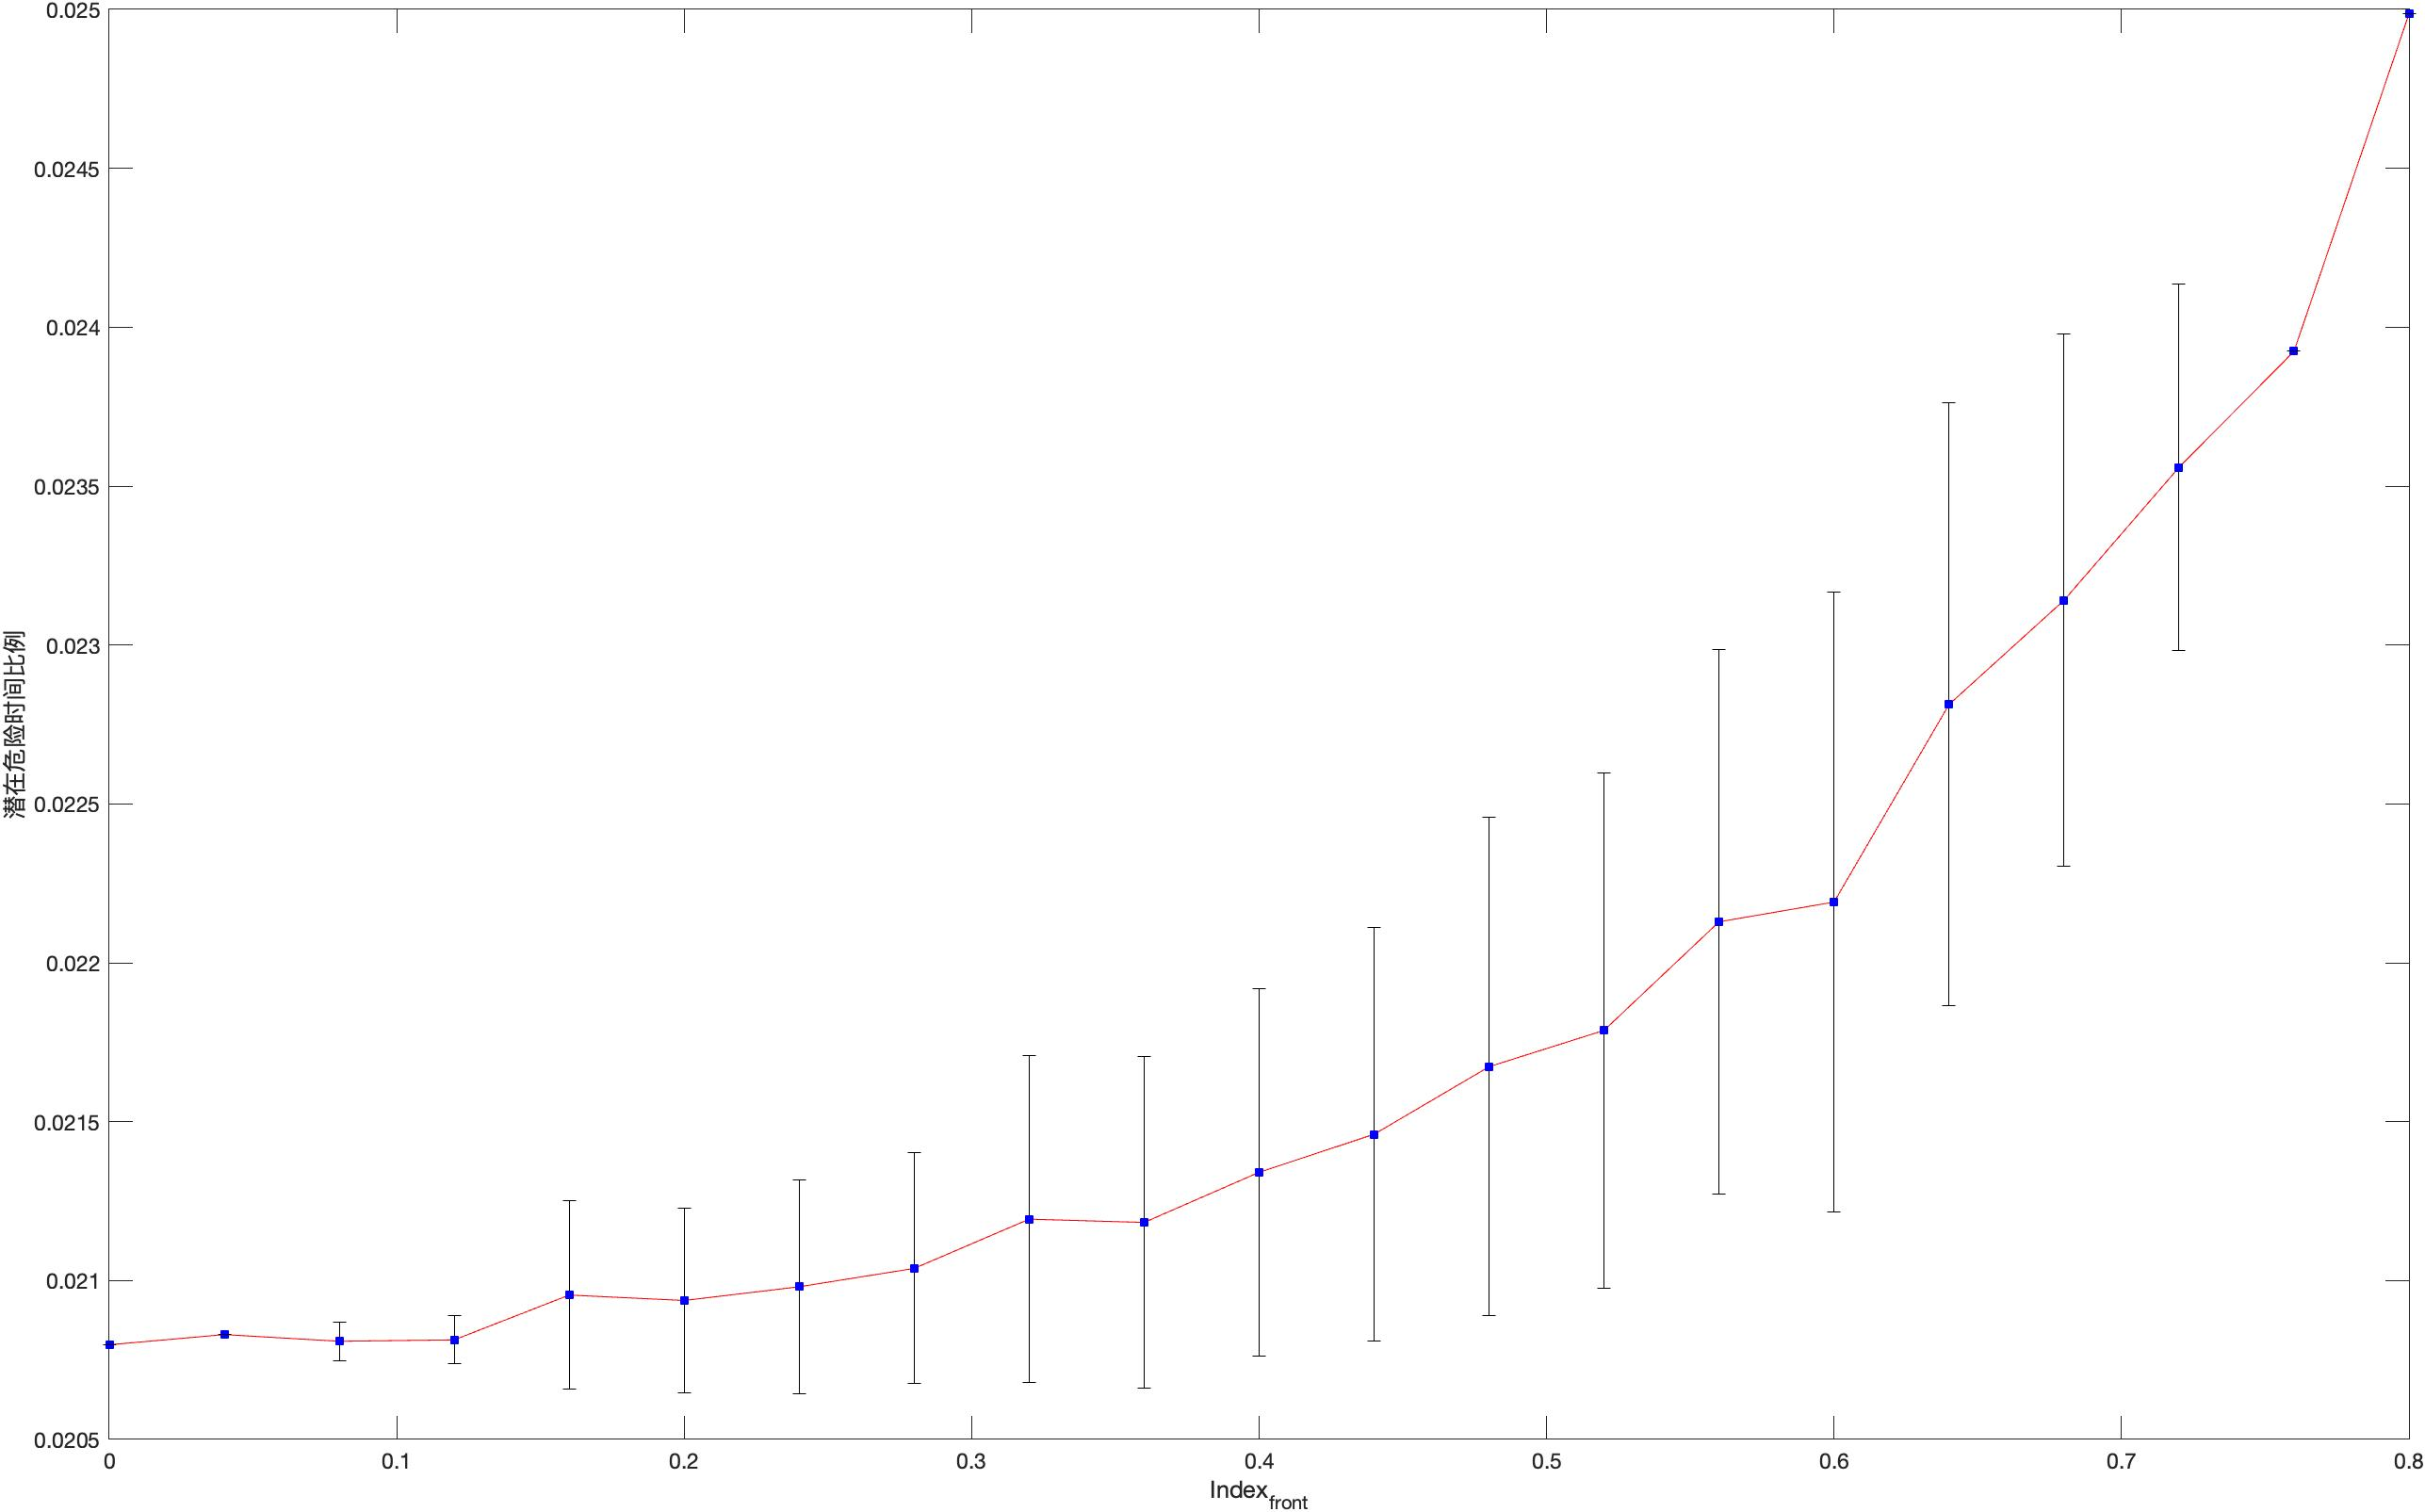
\includegraphics[width=1\linewidth]{chap04-front-PDT.jpg}
    \caption*{Error bar代表标准差}
    \caption{队首聚集度与潜在危险时间比例的关系}
    \label{fig:chap04-9}
\end{figure} 

可以发现二者呈正相关,其Pearson相关系数达到了0.6929。从此图可以看出。队首聚集度越大,自动驾驶车辆整体越远离头车,车队的潜在危险时间比例越大,车队整体越不安全,这与碰撞样本的碰撞风险演化机理是一致的,均呈现出队首聚集度越大,车队整体碰撞风险越大的规律。

图\ref{fig:chap04-9}所示的规律可以解释为:相比于自动驾驶车辆,人工驾驶车辆衰减扰动的能力更强,所以当自动驾驶车辆整体更靠近头车,扰动首先由自动驾驶车辆传递,并不断衰减,当传递到人工驾驶车辆时,扰动的幅度已减小了很多,再通过人工驾驶车辆传递,也不会造成太大的潜在危险。

为了对以上猜想进行验证,我们考虑一个给定排列的车队
\begin{equation}
    \mathrm{AV, AV, AV, AV, AV, HV, HV, HV, HV, HV} \notag
\end{equation}
其中AV代表人工驾驶车队,HV代表自动驾驶车队。仍给定初始均衡速度为$20m/s$观察每辆车的最大扰动,得到\ref{fig:chap04-10}所示结果。

\begin{figure}
    \centering
    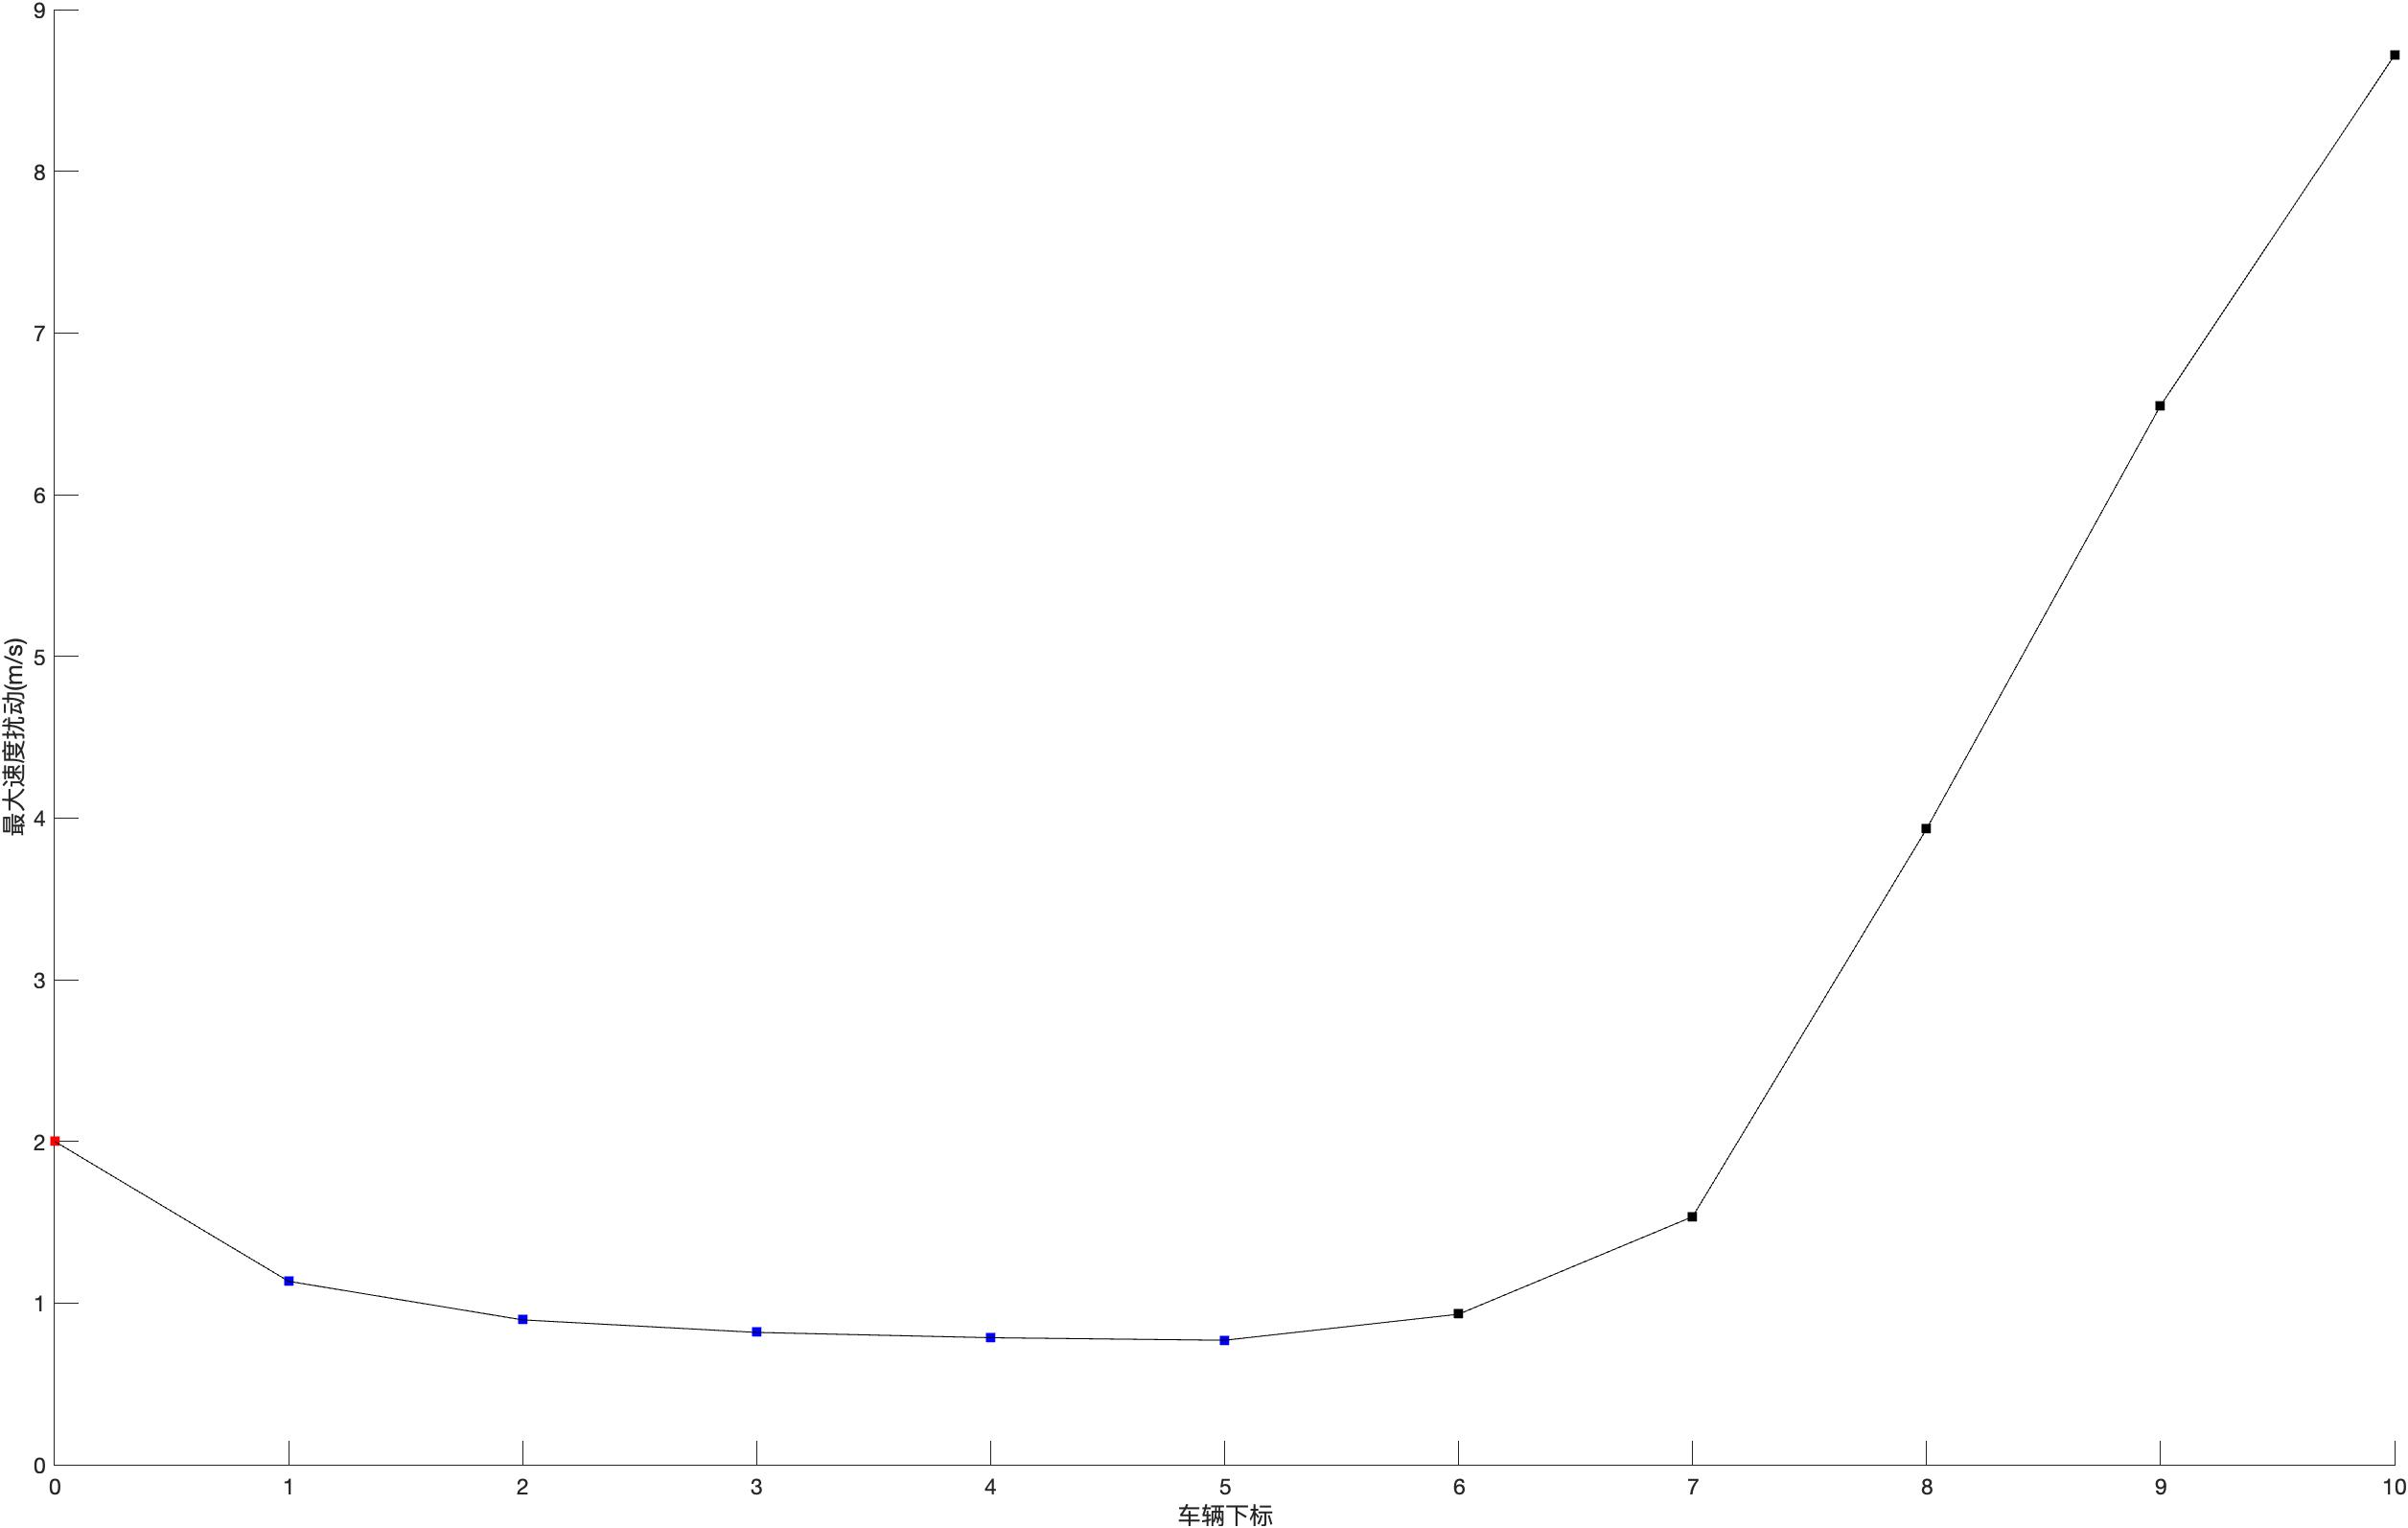
\includegraphics[width=1\linewidth]{chap04-index-delta.jpg}
    \caption*{红色样本点代表头车,蓝色样本点代表自动驾驶车辆,黑色样本点代表人工驾驶车辆}
    \caption{车队中各车最大扰动情况}
    \label{fig:chap04-10}
\end{figure} 

可以观察到对于自动驾驶车辆,即前5辆跟驰车辆,扰动大小呈下降的趋势,说明自动驾驶车辆有衰减扰动的效果,但对于人工驾驶车辆,即后5辆跟驰车辆,扰动被不断放大,这可能也是碰撞风险的主要来源。

\begin{figure}
    \centering
    \subcaptionbox{第3辆车跟驰车辆速度曲线\label{fig:chap04-7-1}}
      {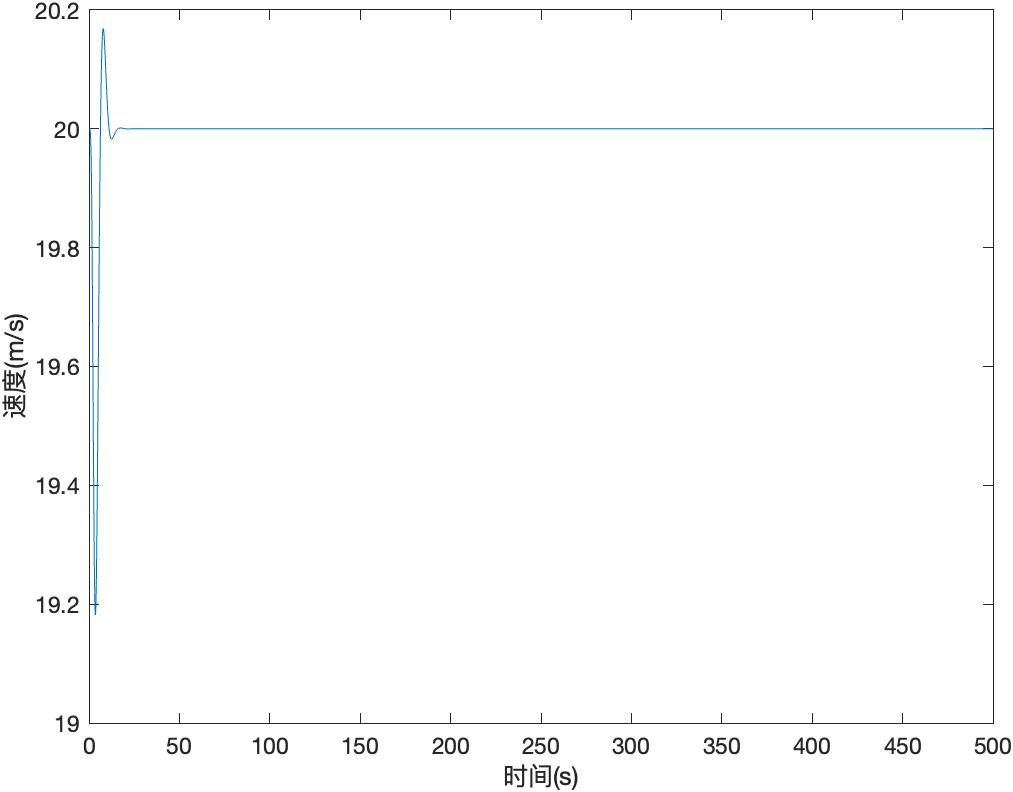
\includegraphics[width=0.49\linewidth]{chap04-3-AV.jpg}}
    \subcaptionbox{第8辆车跟驰车辆速度曲线 \label{fig:chap04-7-2}}
      {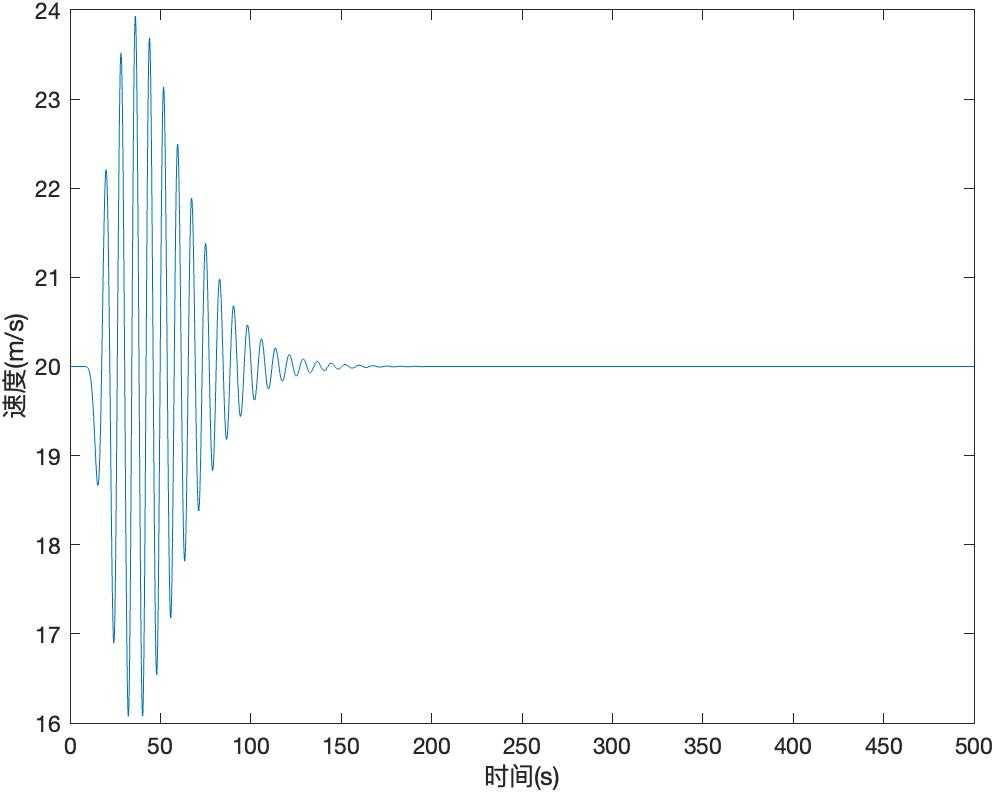
\includegraphics[width=0.49\linewidth]{chap04-car8-HV.jpg}}
      \caption{第3辆和第8辆跟驰车辆速度曲线}
    \label{fig:chap04-11}
  \end{figure}

图\ref{fig:chap04-11}显示了该实验中第3辆车跟驰车辆(自动驾驶车辆)和第8辆跟驰车辆(人工驾驶车辆)的速度曲线。可以发现第3辆车跟驰车辆速度扰动在不断衰减,而第8辆跟驰车辆的速度扰动先增大后衰减,这其实也和二者的稳定性有关,计算二者传递函数的无穷范数得到

\begin{equation}
    \begin{cases}
      \Vert G_{AV}(j\omega) \Vert_{\infty} < 1 \\
      \Vert G_{GV}(j\omega) \Vert_{\infty} > 1
    \end{cases}
    \label{eq:chap04-10}
\end{equation}

这说明虽然车队整体是队列不稳定的,但自动驾驶车辆是稳定的,其速度扰动会不断衰减;而人工驾驶车辆是不稳定的,其速度扰动会先增大,后减小。

即使是将5辆人工驾驶车辆和5辆自动驾驶车辆聚集在一起,5辆人工驾驶车辆跟驰5辆自动驾驶车辆的效果也是不同的,在该实验设定下,前车更为安全,因为在车队的前半段,自动驾驶车辆会先将扰动衰减再传递给人工驾驶车辆。

这样的规律也启示我们,对于真实场景,即使车辆有了不同的跟驰模型,也可以首先分析单车的稳定性,以单车的稳定性指导车队实现更低碰撞风险的排列。

图\ref{fig:chap04-12}所示是潜在危险时间比例与分散均匀度的关系。

\begin{figure}
    \centering
    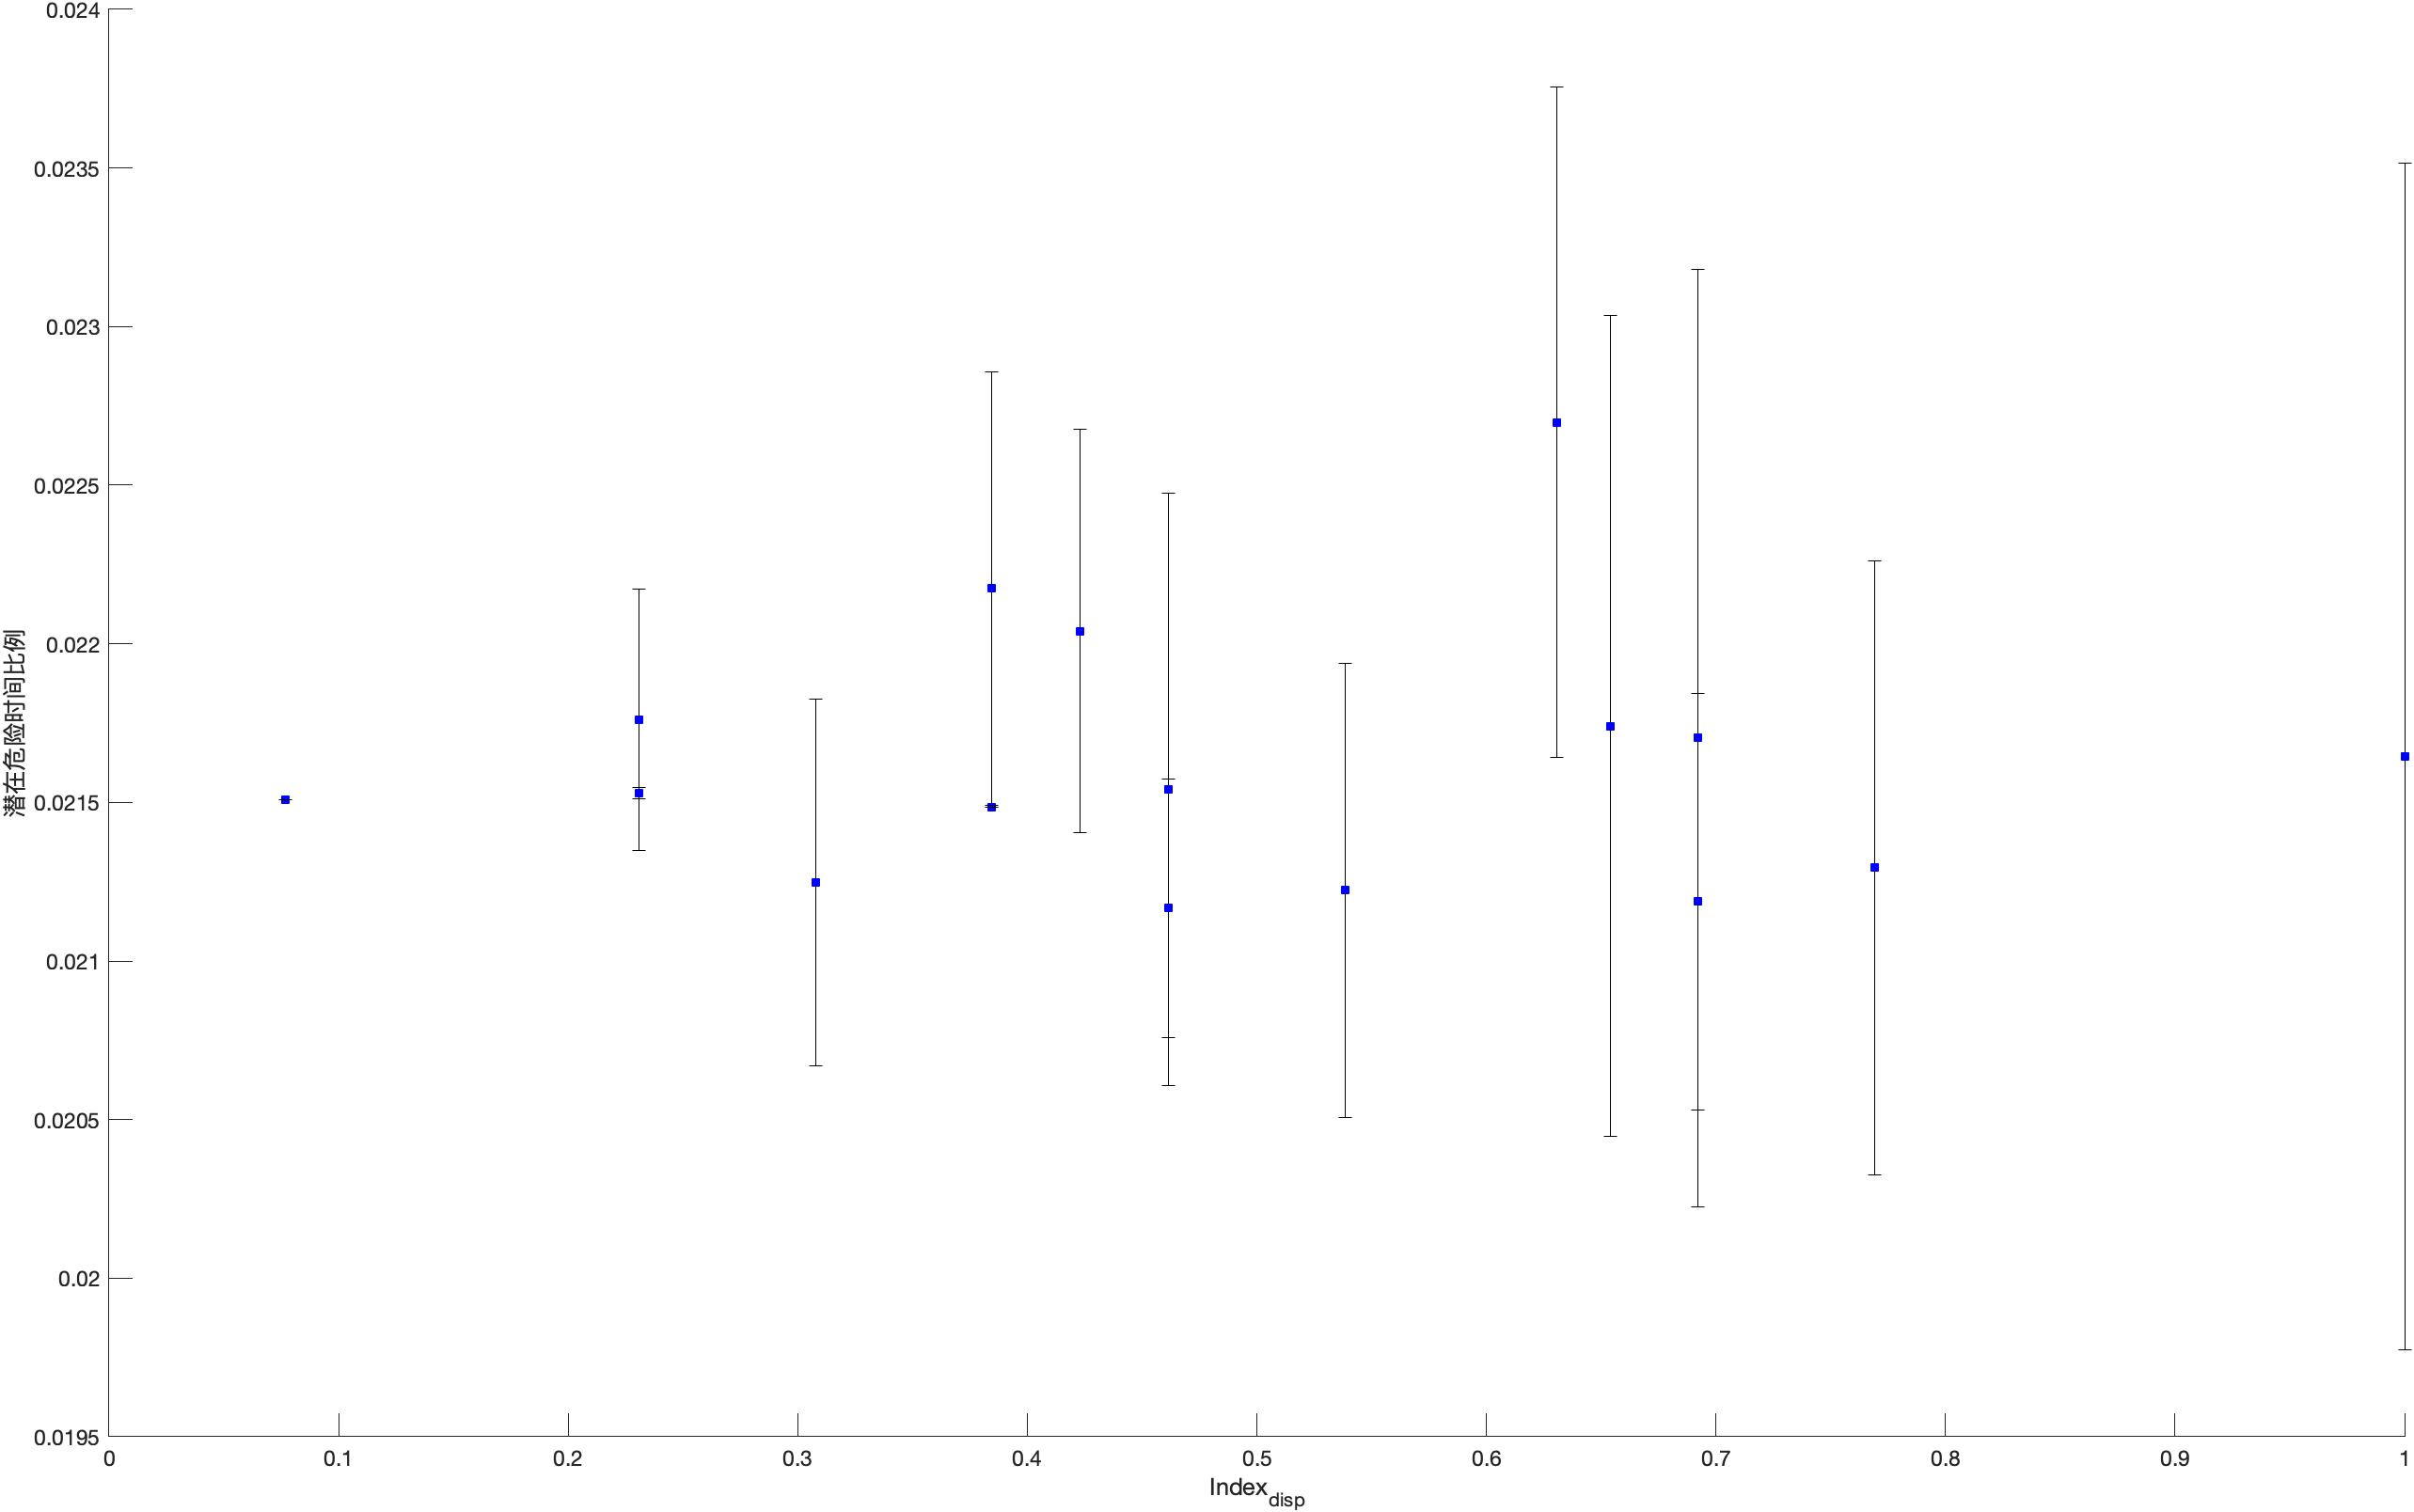
\includegraphics[width=1\linewidth]{chap04-disp-PDT.jpg}
    \caption{分散均匀度与潜在危险时间比例的关系}
    \label{fig:chap04-12}
\end{figure} 

可以发现分散均匀度与潜在危险时间比例并没有明显的关系,这与碰撞样本中二者的情况一致。

\section{本章小结}

在本章中,首先根据是否发生碰撞将实验样本分为了两大类,对于每一类分别选取了稳定性指标和碰撞风险指标。

混合车队的队列稳定性与碰撞风险之间的关系方面,研究发现,对于碰撞样本,车队的队列稳定性越好,碰撞越晚发生,且碰撞越靠近队尾;对于非碰撞样本,车队的队列稳定性越好,车队整体的潜在危险时间比例越低,即车队整体的碰撞风险更小。

混合车队的碰撞风险演化机理方面,首先选择了队首聚集度和分散均匀度这2个车队空间分布指标,研究发现,无论是对于碰撞样本还是对于非碰撞样本,碰撞风险的演化都与队首聚集度有关,而与分散均匀度无明显关系。

图\ref{fig:chap04-strcture}描述了本章的结构。

\begin{figure}
    \centering
    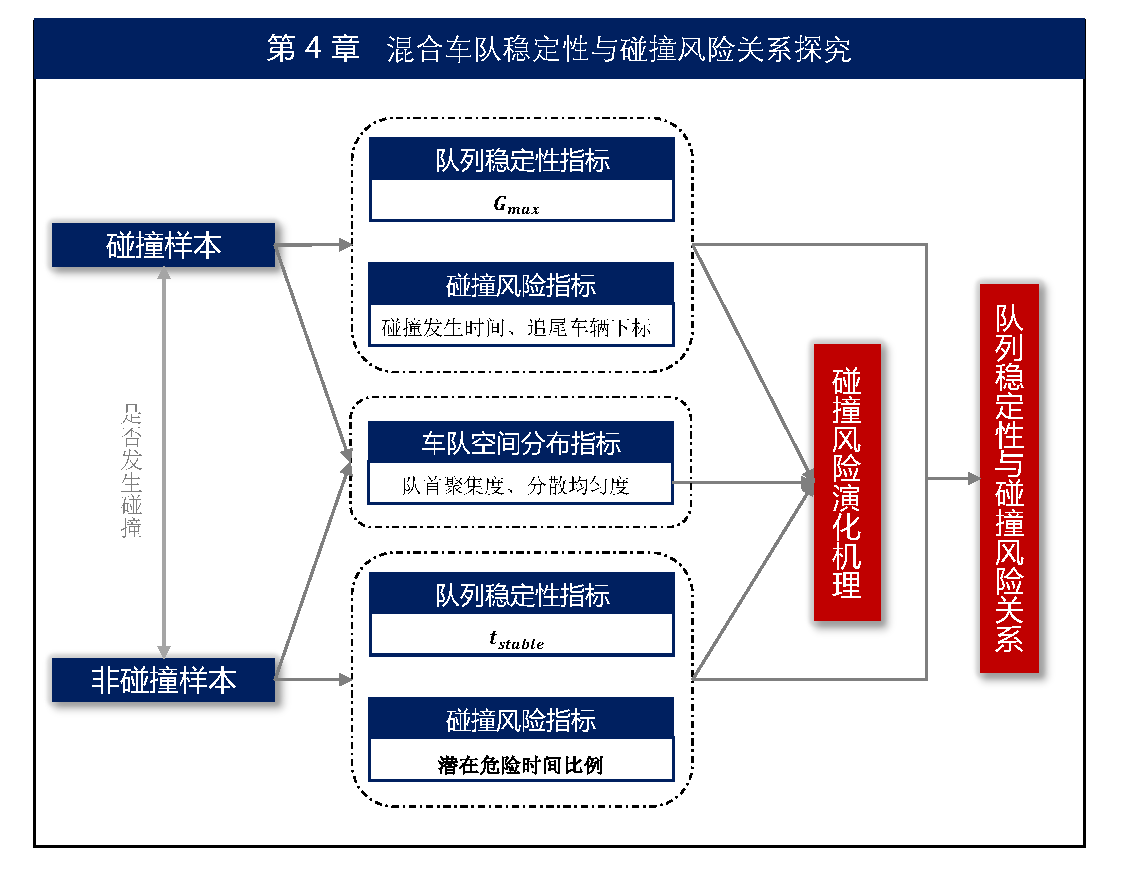
\includegraphics[width=1\linewidth]{chap04-structure.pdf}
    \caption{第4章结构}
    \label{fig:chap04-strcture}
\end{figure} 

